\documentclass[10pt]{article}
\usepackage{color}
\usepackage{graphicx}
\usepackage[T1]{fontenc}
%%% The next two are necessary to get the degree symbol in text and math mode
\usepackage{textcomp}
\usepackage{gensymb}
\usepackage[colorlinks=true,
            urlcolor=cyan]{hyperref}
\usepackage{units}
\usepackage[type1]{libertine}
\usepackage[libertine]{newtxmath}
\usepackage{bm} 

%%% This makes a nice upright greek mu for use in units
\makeatletter
\re@DeclareMathSymbol{\mu}{\mathord}{lettersA}{22}
\makeatother
%%% 
\newcommand{\micron}{\ensuremath{\mu\mathrm{m}}}

\begin{document}
\tableofcontents
\section{Vertex Detector R\&D}
\section{DEPFET Pixel Sensors}

\subsection{The DEPFET Collaboration}
\href{http://www.hll.mpg.de/twiki/bin/view/DEPFET/CollaborationList}{The DEPFET collaboration} consists of nearly 100 members from 13 institutes. It currently takes responsibility for the following work packages:
\begin{description}
\item[Mechanics] {The DEPFET ladder integrates the support structure with the sensor wafer using state-of-the-art silicon processing technology. Read-out electronics and signal routing are integrated on the silicon wafer. The resulting all-silicon ladder is fully self-supporting. The mechanical properties of thin ladders in a realistic environment are studied in detail using detailed models (mock-ups) for Belle II and the ILC .}
\item[Cooling] {The DEPFET cooling concept for Belle II relies on two-phase \ce{CO2} cooling for the end-of-ladder. The sensor is cooled moreover with a forced flow of cold gas. The \ce{CO2} cooling plant is developed by KEK, while the design for the cooling block/support structure is performed within the collaboration. The impact of the linear collider cooling strategy - based on reducing the power dissipated using a pulsed power supply to the detector and cooling through a forced air flow - is studied. A novel cooling strategy for future applications based on mico-channels in the sensors is being evaluated in the collaboration. Solutions for monitoring of environmental parameters are being developed.}
\item[Ancillary ASICs] {The operation of a DEPFET detector requires ancillary electronics in the form of a read-out ASIC (the Drain Current Digitizer), a steering ASIC (SWITCHER) and on-detector ASICs for digital data processing (DHP). These ASICs are developed within the collaboration.}
\item[Data Acquisition and Trigger] {The development of off-detector electronics to process the data from the Belle II vertex detector.}
\item[Characterization of prototypes, laboratory and beam tests] {This work package has contributions from nearly all institutes involved in the DEPFET collaboration.}
\end{description}

Currently, the construction of the Belle II vertex detector~\cite{Abe:2010gxa} is the main focus of the collaboration. The requirements of the Belle II vertex detector are similar to those of the ILC, and more stringent in some aspects. The Belle II construction project therefore has considerable synergy with developments for a future linear collider. The LC-specific effort is focused on the development of small-pixel devices and the design of a forward vertex detector. We envisage that after the installation of the Belle II detector (2016) the balance between both projects is restored.



\subsection{Introduction}
The DEPFET technology implements amplification within the active pixel by integrating a p-MOS transistor in each pixel on the fully depleted high-resistivity silicon wafer. Additional n-implants near the transistor act as a trap for charge carriers created in the substrate (internal gate), so that they are collected beneath the transistor gate. The amplified signal is extracted from the pixel matrix by a numbers of ASICs~\cite{Kishishita:2014maa,Krueger2010337} mounted directly on the sensor: The SWITCHER, Drain Current Digitizer (DCD)~\cite{1748-0221-6-01-C01085,5446501} and Data Handling Processor (DHP)~\cite{1748-0221-7-01-C01069}. 



The DEPFET in-pixel amplification allows for a comfortable signal-to-noise ratio with a very thin active detector. The reduced sensor thickness of 75 $\micron$ for Belle II, 50 $\micron$ for the Linear Collider, is the key to remain within the material budget of 0.15\% of a radiation length per layer. DEPFET prototypes with 20$\times$ 20 $\micron^2$, small enough to meet the stringent spatial resolution specifications of the ILC, have successfully been operated in beam tests~\cite{Andricek:2011zza,Velthuis:2008zza}. The DEPFET matrix is read out in rolling shutter mode at a rate of 100 ns/row. For the column depths relevant for the ILC and Belle II a frame rate of several tens of $\mu$s is achieved~\cite{6484214}. The expected performance of a DEPFET-based vertex detector meets the specifications drawn up by the ILD experiment. DEPFET is also considered as a back-up solution to the SiD concept, in case the single bunch crossing time stamping proves to be out of reach.



\begin{table}
\centering
\caption{Comparison of ILC and Belle II requirements of a vertex detector}
\label{tab:Vertex:DEPFET:ILCBelleComparison}
\begin{tabular}{ccc}
    & ILC & Belle II \\
    \hline
    occupancy & 0.13 hits/$\micron^2$/s & 0.4 hits/$\micron^2$/s \\
    radiation & $< \unit[100]{krad/yr}$ & $> \unit[1]{Mrad/yr}$  \\
    & $\unit[10^{11}]{MeV n_{eq}/yr}$ & $2\times \unit[10^{12}]{MeV n_{eq}/yr}$ \\
    duty cycle & 1/200 & 1 \\
    frame time & $25-\unit[100]{\upmu s} $ & $\unit[20]{\upmu s}$ \\
    momentum range & 100 keV - 500 GeV & $ < \sim\unit[1]{GeV}$ \\
    angular acceptance & 6\degree - 174\degree & 17\degree - 150\degree \\
    spatial resolution & excellent: $3-\unit[5]{\micron}$ & moderate \\
    pixel size & $20\times \unit[20]{\micron}$ & $50\times \unit[75]{\micron}$ \\
    material budget & 0.15\% $X_0$/layer & 0.21\% $X_0$/layer \\
\end{tabular}
\end{table}

\subsection{Recent Milestones}
The concept of a DEPFET active pixel detector for vertex detection at collider experiments was initiated in the linear collider community (for TESLA).
The operation principle was extensively proven~\cite{Andricek:2011zza,Velthuis:2008zza} on small-scale prototypes. A recent reassessment of the DEPFET potential for a linear collider at the energy frontier is found in~\cite{6484214} and in the report~\cite{depfet_ecfa_report} for the ECFA detector R\&D review in 2014.
A large-scale, \unit[75]{\micron} thin Belle II ladder with the ancillary ASICs integrated on the sensor was successfully submitted to a test in an electron beam at DESY in January 2014\cite{Marinas:2014iza}.


The first full-scale DHP prototype was implemented in IBM \unit[90]{nm} CMOS technology. As this technology was discontinued, more recent designs were submitted in the TSMC \unit[65]{nm} CMOS process. DHPT v.1.0 comprises temperature independent current references, 11 bias 8-bit DACs with current output, an integrated temperature measuring system and JTAG control. This design has been successfully tested during early 2014\cite{Kishishita:2014maa}.

\subsection{Engineering Challenges}
Vertex detector ladders with a thickness of several tens of microns and a spatial resolution of well below \unit[10]{\micron} require very robust mechanical properties. The power generated by the sensors and ASICs must be removed with the smallest impact on the detector material.
Measurements on thin ladders under a realistic load, including pulsed powering according to the ILC beam structure, prove the excellent mechanical properties of the all-silicon ladder~\cite{thermomech}.

\subsection{Future Plans}
Currently, the construction of the Belle II vertex detector (to be installed by 2016 for the first physics run in 2017) implies a large effort of R\&D, including:
\begin{itemize}
\item Develop the die-attach technology in a controlled atmosphere required for the mounting of passive components on the DEPFET active pixel detector ladders. The first milestone is a fully integrated electrical prototype based on the EMCM.
\item First tests that will determine if all the ASICs on the ladder are fully functional
\item The integration of read-out and steering ASICs on the pixel sensor to be performed using a flip-chip technique and so-called bump-bonding, using microscopic solder balls.
\item The production of the Belle II vertex detector modules, a joint effort of the DEPFET collaboration
\item The test of the last version of the DHP chips
\end{itemize}
In the near future we hope to characterize the performance of a thin ILC-design prototypes with pixels of $20 \times \unit[20]{\micron^2}$
\begin{itemize}
\item Perform an engineering design for a DEPFET all-silicon module with the required petal geometry
\item A detailed characterization of the response of the device
\item Design of the ancillary ASICs, taking full responsibility for future design cycles of the Front End read-out chip, the Drain Current Digitizer (DCD) that is relevant to the ILC and a Belle II upgrade. This chip converts the analog signal from the detector to digital and has a crucial impact on the detector performance.
\end{itemize}

In the longer term the DCD and DHP are envisaged to evolve into a single chip. Being large arrays of DEPFET pixels a promising technology for the vertex detector of the planned ILC, adaptation of the DCD and DHP chips must also be done.

 In the near future we hope to characterize the performance of ILC design prototypes with pixels of $20 \times \unit[20]{\micron^2}$.
Important experience is furthermore gained with the thermal and mechanical properties of ultra-thin ladders. Measurents on thin ladders under a realistic load, including pulsed powering according to the ILC beam structure, prove the excellent mechanical properties of the all-silicon ladder. A complete mock-up for the innermost disks is under construction.

\subsection{Applications Outside of Linear Colliders}
The concept of a DEPFET active pixel detector for vertex detection at collider experiments was initiated in the linear collider community (for TESLA). The election of DEPFET technology for the Belle II detector therefore represents an important spin-off of linear collider detector R\&D. DEPFET is also considered a strong candidate technology for the vertex detector at a future circular collider (http://cepc.ihep.ac.cn/preCDR/volume.html). DEPFET detectors are furthermore used for X-ray imaging at the XFEL~\cite{xfel}. Future space missions envisage the use of DEPFET sensors~\cite{bepicolombo}. Their use in microscopy is being studied.





\section{ChronoPixel}

\subsection{Introduction}
The ChronoPixel is a monolithic CMOS pixelated sensor with the ability to record up to two time stamps of pixel hits by charged particles in a nominal ILC bunch train. This information is read out in the time interval between bunch trains. The ChronoPixel option for the ILC vertex detector was described in the ILC DBD~\cite{2011arXiv1109.2811B}. By the time of the DBD, 2 prototypes had been built and tested, and the summary of test results was also presented in the DBD. The main points are:
\begin{figure}
    \centering
    \begin{minipage}[t]{0.49\textwidth}    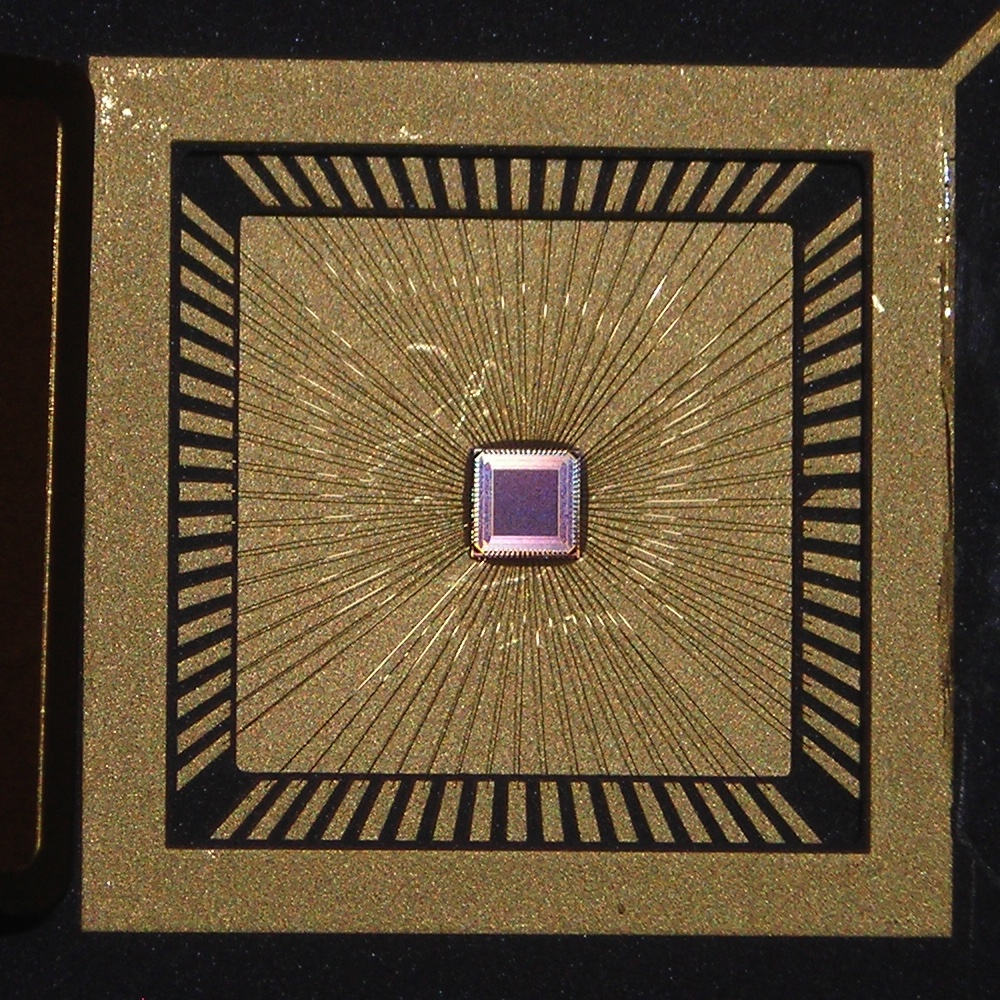
\includegraphics[width=\linewidth]{VertexDetector/Chronopix/Chronopix_image}
    \caption{Photograph of the prototype 3 chip in its package. The chip has $48\times48$ pixels, each with a size of $25\times\unit[25]{\micron^2}$.}
    \label{fig:VertexDetector:ChronoPixel:image}
\end{minipage}\hfill
\begin{minipage}[t]{0.49\textwidth}
    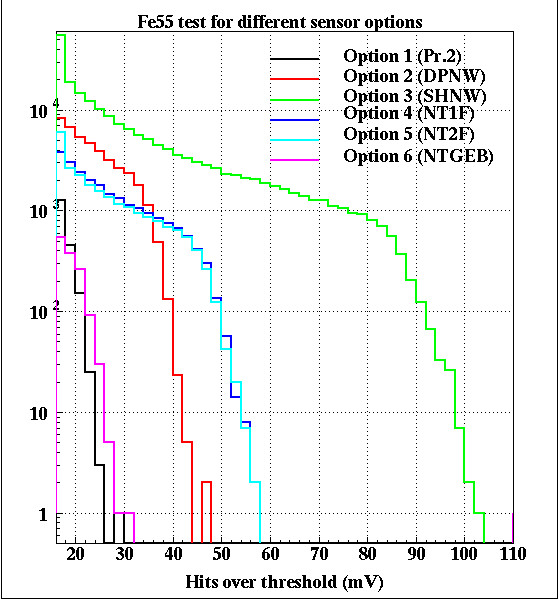
\includegraphics[width=\linewidth]{VertexDetector/Chronopix/Fe55tst}
    \caption{\ce{^{55}Fe} signal over threshold counts for 6 different sensor diode options,
implemented in prototype 3. For comparison, option 1 is the same as in prototype 2.}
    \label{fig:VertexDetector:ChronoPixel:Fe55Response}
\end{minipage}
\end{figure}
\begin{itemize}
    \item We have proven that we can record time stamps in every pixel with time resolution down to \unit[150]{ns}.
    \item We have tested sparse readout, allowing to read only pixels with hits, thus reducing readout time to the level allowing readout of all pixels in the sensor in the intervals between bunch crossings.
    \item We have tested pulsed power for the analog part of the pixels and have proven~\cite{sinev:Chronopix:FirstPrototype} that turning power ON about \unit[100]{$\mu$s} before bunch train and turning it off between bunch trains does not create any problems for threshold setting accuracy in the comparators.
    \item We have measured sensor noise level, including all pick-up and cross-talk. It was 24 e- r.m.s in prototype 1 and 26 e- r.m.s. in prototype 3, sensor option 3. Our specification was 25 e-.
noise.
    \item We have tested the idea of building all in-pixel electronics only from NMOS transistors, thus eliminating the need for a special process (deep p-well) to protect signal charge from parasitic collection by in-pixel transistors. We have proven~\cite{sinev:Chronopixel:RnDstatus2013} that all NMOS electronics can be built in this way, and that this does not significantly increase the power consumption compared to CMOS electronics.
    \item We have tested the compensation of comparator offsets using analog calibration, when the value of the offset is stored as a voltage on the capacitor in each pixel. This has an advantage over digital calibration (where the offset value is stored as code in the special register) in that there are no discrete levels, and the accuracy of such a calibration scheme is not affected by the size of the register or the spread of the initial offsets.
\end{itemize}
\subsection{Recent Milestones}
\begin{itemize}
    \item Test of prototype 2 revealed some problems. Possible solutions for these problems were discussed with Sarnoff engineers.
    \item A new contract with Sarnoff for the design of prototype 3 was signed in August 2013.
    \item Prototype 3 was manufactured in September 2014. Tests have shown that problems revealed in prototype 2 were solved.
\end{itemize}
The most recent report~\cite{sinev:POS:Vertex2105} on the status of ChronoPixel was presented by N.~Sinev in June 2015 at Vertex2015 in Santa Fe, New Mexico.

\subsection{Engineering Challenges}
\begin{itemize}
    \item The Vertex Detector for ILC faces many engineering challenges. The sensors need to be thinned to about \unit[50]{\micron} to reduce the amount of material in the detector. Support structures also need to be very light, but provide enough stability. Power dissipation of the entire detector should be small to be able to use only air cooling.
    \item If acceptable levels of the sensor diode capacitance can be achieved, the signal-to-noise ratio will improve. However, a lower value of the capacitance will make the pixels more sensitive to cross-talk through capacitive coupling. Reducing this coupling can be a challenge.
    \item Transition from small prototypes (few $\text{mm}^{2}$) to ILC detector size ($\approx \unit[10]{cm^2}$) may meet additional problems. One of them will be the effect of Lorentz forces on the power supply buses, especially in the case of power pulsing. Power pulsing is the only way to achieve acceptable power dissipation in the vertex detector. However, it will generate varying Lorentz forces, acting on power supply lines. This may produce vibrations, which are unacceptable for the required spatial resolution of the detector.
\end{itemize}

\subsection{Future Plans}
\begin{itemize}
    \item To achieve signal-to-noise ratio required for close to 100\% signal registration efficiency. We have achieved very low sensor capacitance in prototype 3, and the signal-to-noise ratio with such a sensor capacitance for \ce{^{55}Fe} signal is about 60, however, for minimum ionizing particles the signal will be much smaller, depending on epitaxial layer thickness and charge collection efficiency. The signal-to-noise ratio for standard \unit[7]{\micron} epitaxial layer will be 20 if the charge collection efficiency is 100\%, which is unlikely (we have not measured it yet). So we probably will need to increase the epitaxial layer thickness.
    \item To achieve the required pixel size (prototype 3 has \unit[25]{\micron} pixels, we would eventually like \unit[15]{\micron}). It may require going to a technology with feature size less than \unit[65]{nm}. There seems to be no problems in that, but both -- good signal-to-noise ratio and pixel size requirements may be challenging.
    \item To achieve acceptable level of inter-pixel and digital-to-analog circuit cross talks and parasitic feedback.
    \item Depending on available funding, to build a complete sensor with a large enough area and full feature readout.
\end{itemize}

\subsection{Applications Outside of Linear Colliders}
     With some modifications (for example, adding time-time converter) ChronoPixel architecture can be applied for any experiment requiring time stamping of individual hits -- it may be HL-LHC, CLIC and so on.

\section{FPCCD}
\subsection{Collaborating Institutions}
\subsection{Introduction}
    Fine pixel CCD (FPCCD) is one of the candidate sensor options for the vertex detector of the ILD detector at the ILC~\cite{Sugimoto:2005ru,2009arXiv0902.2067S,2012arXiv1202.5832S}. In the present design, FPCCD sensors for the innermost layer of the vertex detector have a pixel size of \unit[5]{\micron} and a fully depleted epitaxial layer with a thickness of \unit[15]{\micron}. Because of the small size of the pixels, the occupancy is acceptably low even if the hits are accumulated for one nominal ILC bunch train ($\approx\unit[1]{ms}$).
    The efforts of the FPCCD collaboration are currently focused on pixel characterization and development, while we also pursue developments to the cooling system, electronics downstream of ASICs and the reconstruction software~\cite{Mori:2014xta}.
\subsection{Recent Milestones}
R\&D activity for the FPCCD vertex detector at present is mainly focused on FPCCD sensors and a detector cooling system using 2-phase \ce{CO2}.
One of the achievements of FPCCD sensors after DBD is the fabrication of real size ($12.3 \times \unit[62.4]{\mathrm{mm}^2}$) sensors with \unit[50]{\micron} total thickness. Figure~\ref{fig:FPCCD:realSizeSensor} shows the real size prototype sensor. It has 8 readout nodes, and each channel has different pixel sizes of \unit[12]{\micron}, \unit[8]{\micron}, and \unit[6]{\micron}.
\begin{figure}
 \begin{minipage}[t]{0.49\textwidth}
\centering     \includegraphics*[width=\textwidth,keepaspectratio]{VertexDetector/FPCCD/realSizeFPCCDSensor.png}
    \caption{Real size FPCCD sensor thinned down to \unit[50]{\micron}}
    \label{fig:FPCCD:realSizeSensor}
 \end{minipage}
 \hfill
 \begin{minipage}[t]{0.49\textwidth}
 \centering
    \includegraphics*[width=\textwidth,keepaspectratio]{VertexDetector/FPCCD/coolingSystemSchematic.png}
    \caption{A simplified schematic diagram of the two-phase $\text{CO}_2$ cooling system}
    \label{fig:FPCCD:coolingSystemSchematic}
 \end{minipage}
 \end{figure}

We have started a neutron damage test using small ($\unit[6]{mm}\times\unit[6]{mm}$) FPCCD prototypes~\cite{lcws:fpccd:ito:2013}. A prototype sensor was irradiated by a neutron beam of few tens of MeV at the CYRIC facility of Tohoku University. The detailed analysis on the irradiated sensor is still on-going.
In order to increase the radiation immunity of FPCCD sensors, particularly to reduce the transfer inefficiency due to radiation damage, the sensors should be cooled down to \unit[-40]{\degree C}. We have started R\&D on a two-phase \ce{CO2} cooling system for this purpose. There are several examples of utilizing two-phase \ce{CO2} cooling systems for high energy physics experiments. For these cases, the \ce{CO2} coolant is circulated using liquid pumps. This method is, however, not so efficient for very low temperature cooling of \unit[-40]{\degree C}. Therefore, we adopted a \ce{CO2} gas compressor for the circulation of \ce{CO2} coolant. Figure~\ref{fig:FPCCD:coolingSystemSchematic} shows a simplified schematic diagram of the system. A prototype system has been constructed, and cooling between \unit[-40]{\degree C} and \unit[+15]{\degree C} has been successfully demonstrated using this system.

\subsection{Engineering Challenges}
    In the present design of the ILD vertex detector, two sensor layers are mounted on both sides of a light-weight ladder of ~\unit[2]{mm} thickness. Our goal of the material budget of this ladder is 0.3\% X0/ladder = 0.15\% X0/layer. This goal would not be so easy to accomplish, and we need a lot of R\&D effort.
    The ladders have to be cooled down to \unit[-40]{\degree C}. We plan to achieve this cooling by heat conduction to the end-plate on which thin cooling tubes for 2-phase \ce{CO2} are attached. The design of this structure is not trivial, and we need R\&D including thermal simulation.
    There are challenges both with the mechanical structure and the electronics circuit for the ladder R\&D. We have not started this effort yet.
\subsection{Future Plans}
    We have been doing our R\&D on the FPCCD vertex detector based on a Grant-in-aid for science research which expires at the end of FY2015. By that time, we plan to carry out the following R\&D items:
\begin{itemize}
    \item Characterization of FPCCD sensors including beam tests and radiation damage tests
    \item Development of FPCCD sensors with the pixel size of \unit[5]{\micron}, which is our ultimate goal
    \item Construction of prototype ladders for inner layers
    \item Development of readout electronics downstream of ASICs
\end{itemize}
If new funding is secured in future, the following R\&D items have to be done:
\begin{itemize}
    \item Development of larger FPCCD sensors and prototype ladders for outer layers
    \item Development of readout electronics which can fit in the small space of real experiment
    \item Construction of a real size engineering prototype and its cooling test
\end{itemize}

\subsection{Applications Outside of Linear Colliders}
    Because of the relatively slow readout speed, the application of FPCCD sensors to other high energy physics experiments would be limited. However, high spatial resolution of small pixel size must be applicable to measurements of X-ray imaging.
    Two-phase \ce{CO2} cooling system can be applied to any other detectors which require efficient cooling between \unit[-40]{\degree C} and near room temperature. Our system, which uses a \ce{CO2} gas compressor, has a great advantage for low temperature operation near \unit[-40]{\degree C} compared with systems using liquid pumps for circulation.

\section{CMOS}
\subsection{Introduction}
CMOS Pixel Sensors (CPS) combine high granularity with low material
budget and allow integrating the full signal processing circuitry on
the sensor substrate. Being moreover cost effective because of the
underlying industrial market, CPS are attractive for a wide range of
applications. They are developed for the ILC since more than fifteen
years and were shown to rather easily comply with the required spatial
resolution and material budget of an ILC vertex detector and their
radiation tolerance was observed to go well beyond the ILC requirements~\cite{Behnke:2013lya}. The state of the art of the technology is illustrated
by the 400 ULTIMATE sensors  operated in the STAR-PXL detector~\cite{Greiner201168}
at RHIC/BNL since 2014 and by the 10-100 times faster
sensors developed for the upgrade of the ALICE Inner Tracker System
(ITS)~\cite{0954-3899-41-8-087002}.

The achieved read-out speed of the CPS developed for an ILC
vertex detector is already quite satisfactory~\cite{Behnke:2013lya},
but is worth
improving in ordre to facilitate track seeding at nominal ILC
running conditions and to introduce a safety margin reflecting the
uncertainties affecting the predicted beam related background rate.

The technology should in fact allow single bunch tagging, provided power
consumption and, in turn, power cycling remain under control. The flexibility and detection performances of CPS are also indicating attractive perspectives for trackers, where relaxed constraints on the granularity may be exploited
to find a well suited balance between speed, power saving and material budget. Ambitious goals for an ILC experiment may therefore be considered
since their development may be carried out for numerous years until the design
inputs of a vertex detector ought to be fixed.

The charged particle detection performances of CPS are
currently essentially limited by manufacturing parametres.
The latter evolve steadily since several years in a direction which makes
them increasingly suited to the ILC vertexing and tracking. Besides
achievements targetted with existing processes, the present R\&D
addresses also improvements expected from the evolution of the CMOS
industry, mainly driven by the trend towards smaller feature sizes which
would allow overcoming the conflict between the spatial resolution and the
bunch tagging capability of CPS. This evolution is already well visible
when comparing the performances achieved with the $\unit[0.35]{\mu m}$ process
used for the STAR-PXL and the more recently addressed $\unit[0.18]{\mu m}$ process
used for the ALICE experiment.


The R\&D adresses presently four objectives :
\begin{itemize}
\item 2 or 3 CPS variants optimised for the different vertex detector layers :
\begin{itemize}
\item inner layer : design privileging spatial resolution and read-out speed
\item outer layers : design privileging power saving, exploiting the
				less demanding spatial and time resolutions
\end{itemize}
\item CPS adapted to tracking sub-systems, based on large pixels and privileging
power saving
\item ultra-light double sided ladders (called PLUME~\cite{Nomerotski2011208})
equipped with (identical or complementary) CPS on its two faces
\end{itemize}


\subsection{Recent Milestones}
Specific CPS are being developed since 2011 to equip the Inner Tracking
System (ITS) of the ALICE experiment in the framework of its upcoming
upgrade. The surface to cover exceeds 10 square meters, i.e. nearly two
ordres of magnitude more than the STAR-PXL or an ILC vertex detector.

Two CPS are being developed, differing by their read-out architectures.
The most conservative of them, called MISTRAL-0, reproduces the ULTIMATE
sensor equipping the STAR-PXL and is thus based on a synchronous, rolling-shutter, read-out. The concept underlying the other sensor, called ALPIDE, features an asynchronous read-out based on a token ring relying on a pre-amplifier/shaper/discriminator chain implemented in the pixel array. It
allows for a few microsecond read-out time and for a power consumption below
$\unit[50]{mW/cm^2}$. These performances were demonstrated in 2014~\cite{1748-0221-10-03-C03030}
on a real scale prototype.

MISTRAL-O relies on large pixels to achieve a $\unit[20]{\mu s}$ read-out
time and a power consumption below $\unit[100]{mW/cm^2}$ while providing
$\unit[10]{\mu m}$ resolution with its integrated binary encoding.
Its read-out architecture was validated in 2014 with a real scale
prototype~\cite{Winter:NSSMIC:2014} featuring 160,000 small ($22\times\unit[33]{\mu m^2}$
large) pixels. More recently \cite{Winter:ALCW15}, prototypes composed of
three times larger pixels were tested on beam and demonstrated satisfactory
charged particle detection performances at
30\textdegree C and after radiation loads exceeding those expected at the
ILC by several ordres of magnitude.

In summary, the full chain of the ULTIMATE sensor has been reproduced
in a $\unit[0.18]\{mu m}$ process with twice faster read-out frequency and
improved sensitive volume (epitaxial layer) characteristics. The
optimisation of this design for tracking systems, using relatively
large pixels, is validated.

Moreover, a small prototype of a sensor optimised for the vertex detector
outer layers was realised in the $\unit[0.18]{\mu m}$ process mentioned earlier.
Low power is achieved using enlarged, $\unit[35]{\mu m}$ pitch, square pixels and the
spatial resolution is kept below $\unit[4]{\mu m}$ by integrating a 3-bit ADC in
each pixel. The approach was validated in the former $\unit[0.35]{\mu m}$ process
with the MIMOSA-31 prototype, but the ADCs had to be kept at the sensor
periphery because of process limitations, translating into larger
power consumption and slower read-out. Laboratory tests of the new
prototype were performed since last Summer, showing satisfactory noise performances at nominal read-out speed, thus validating the concept.


\subsection{Engineering Challenges}
Squeezing the material budget of the double-sided PLUME ladders
below $\unit[0.3\%]{X_0}$ will the main engineering challenge, as the design
has to account for the necessity to power pulse the ladders in the
strong experimental magnetic field. Power pulsing seems mandatory
in case of continuous read-out as the sensor design is unlikely to
end up with a power density suppressed enough to avoid switching
the sensors off inbetween consecutive trains. The possibility to
introduce micro-channel cooling in the ladders will be studied in
ordre to mitigate the power pulsing requirements.

\subsection{Future Plans}

Several development directions will be pursued in the coming years,
to improve the performances of the CPS and to assess the added value
of the ultra-light double-sided ladder concept.

The development of CPS will mainly aim at realising a prototype of
a new sensor series, called IBISCUS\footnote{standing for {\bf I}lc
{\bf B}unch {\bf I}dentifying {\bf S}ensor {\bf C}ompatible with
{\bf U}ltraprecise {\bf S}patial resolution},
composed of pixels with less than $\unit[20]{\mu m}$ pitch providing a
read-out time of about $\unit[1]{\mu s}$ (using a token ring read-out).

The R\&D on the other CPS versions mentioned earlier (for the vertex
detector outer layers and for tracking sub-systems) will be pursued
with coarser priority.
Besides these continuous read-out architectures, a sensor composed
of $\unit[4]{\mu m}$ pitch square pixels with analog output, foreseen to be
read out inbetween trains like FPCCDs, will also be studied.

% Studies have shown \cite{1748-0221-10-03-C03030} that the track reconstruction
% would still improve if the sensors could separate individual bunch
% crossings, thus

Different versions of double-sided ladders will be realised and
their performances evaluated in terms of spatial accuracy, including
alignment issues, and in terms of stability against power pulsing,
possibly in a high magnetic field.

The two main alternative design options are going to be compared
to each other. One version is based on a high precision sensor
($<\unit[3]{\mu m}$) on one side featuring $\lesssim\unit[50]{\mu s}$ integration
time, while a fast sensor ($\sim\unit[2-3]{\mu s}$) equips the other side
which provides $\sim\unit[5]{\mu m}$ resolution. The other version is based
on a single sensor equipping both ladder sides, which offers $\sim\unit[4]{\mu m}$
spatial resolution and about $\unit[5]{\mu s}$ time resolution.

\subsection{Applications Outside of Linear Colliders}
CPS developed at IPHC in perspective of the ILC are used in several
devices, as illustrated by the non-exhaustive list below:
\begin{itemize}
\item Several high precision transparent beam telescopes, adapted to
	($<\unit[1]{GeV}$) electron beams, are equipped with the MIMOSA-26 or
	-28 (alias ULTIMATE) sensors
\item The first generation of sensors with full on-chip signal processing
	developed at IPHC (in a $\unit[0.35]{\mu m}$ CMOS process) was applied to the
	STAR-PXL detector at RHIC, which completed successfully its first
	data campaign in 2014 and has started its 2015 run
\item The upgraded ALICE ITS will be the next equipment based on CPS;
	it will provide insight of a token ring architecture pioneering
	the one considered for the IBISCUS chip mentioned above; it will
	also provide running experience with a tracker based on CPS
\item The Micro-Vertex Detector of the CBM experiment at FAIR/GSI will
	also be based on the CPS presently developed for the ALICE-ITS
	upgrade
\item The sensors were, or are, being applied outside of subatomic physics.
	They were for instance used in the FIRST experiment at GSI, for
	hadrontherapy monitoring; they are presently developed for soft
	X-Ray imaging and brain-imaging.
\end{itemize}

Sensors featuring pixels about 5 times larger than those equipping the STAR-PXL were fabricated in 2014, with different pixel design optimisations. Such large pixels are more exposed to the effects of signal charge recombination. The purpose of the paper is, among others, to show that the charge particle detection efficiency is not degraded, even after radiation loads representative of upcoming trackers, such the upgraded ALICE Inner Tracking System. The charged particle detection performances of these large pixel CPS prototypes with integrated signal processing and binary outputs were studied by exposing the sensors to a 450 MeV electron beam. The results obtained will be exposed
and shown to validate the concept for its evolution towards large area tracking devices, with the perspective of integrating logical strips in the sensor.

\section{CLICpix}
% \subsection{Collaborating Institutions}
% The vertex-detector R\&D for CLIC is carried out in the framework of the CLIC detector and physics
% collaboration (CLICdp), presently composed of 25 institutions~\cite{CLICdp-collaboration}.
% The main contributors to the vertex-detector
% project are
% Cambridge University,
% CERN,
% University of Geneva,
% Karlsruhe Institute of Technology (KIT),
% University of Liverpool,
% SLAC,
% Institute of Space Science Bucharest and the
% Spanish Network for Linear Colliders

\subsection{Introduction}
 The precision physics needs at the CLIC TeV-scale linear electron-positron collider
require a vertex-detector system with excellent flavour-tagging capabilities through
a measurement of displaced vertices in an environment with high rates
of beam-induced background events~\cite{Miyamoto:1425915}.
As a result, the CLIC vertex-detector system needs to have excellent spatial resolution
(\unit[3]{\micron}),
full geometrical coverage extending to low polar angles, extremely low material budget
(0.2\% $X_0$ per layer),
low occupancy facilitated by time-tagging (\unit[10]{ns} precision), and sufficient heat
removal from sensors and readout.
A concept based on hybrid pixel-detector technology is under development
for the CLIC vertex detector. It comprises fast, low-power and small-pitch readout
ASICs implemented in \unit[65]{nm} CMOS technology (CLICpix) coupled to ultra-thin planar sensors
or active HV-CMOS sensors via low-mass interconnects. The power dissipation of the
readout chips is reduced by means of power pulsing, allowing for a cooling system
based on forced gas flow. Through-Silicon Via (TSV) vertical interconnects remove the need for wire
bonding connections on the side of the readout ASICs
and therefore allow for an efficient tiling to form larger modules with minimal
inactive areas.
\subsection{Recent Milestones}
A broad hardware R\&D program is in place, addressing the challenges for the CLIC
vertex detector in an integrated approach~\cite{1748-0221-10-03-C03025}. Recent achievements
in the sensor and readout domain include:
\begin{description}
\item[Hybrid pixel assemblies with ultra-thin planar sensors]
Planar pixel sensors with \unit[55]{\micron} pitch and different thicknesses (\unit[50--300]{\micron})
were procured from different vendors and bump-bonded to Timepix~\cite{Llopart2007485} readout
ASICs (100 and \unit[700]{\micron} thickness).
Slim-edge sensor designs are compared to designs
with active edges.
Preliminary beam-test results show very good efficiencies in both cases, extending beyond the
edge pixels~\cite{Redford:1966932}.
For \unit[50]{\micron} sensor thickness and nominal readout parameters, the fraction of multi-pixel clusters
is approximately 20\%.
Single-point resolutions of approximately \unit[3]{\micron} have been extracted
for clusters of two pixels using charge interpolation and taking into account
non-linear charge sharing.
\item[CLICpix demonstrator ASIC]
A CLICpix demonstrator chip has been produced in \unit[65]{nm} CMOS technology,
including a $64 \times 64$ pixel matrix and power-pulsing capability~\cite{Valerio:1507691}.
The pixel size is $\unit[25]{\micron}\times\unit[25]{\micron}$. Simultaneous
4-bit Time-Of-Arrival (ToA) and Time-Over-Threshold (ToT) measurements
are implemented in each pixel, allowing for a front-end time slicing
with approximately \unit[10]{ns} and for measuring the charge
to improve the position resolution through interpolation.
The full chip can be read out in less than
$\unit[800]{\upmu s}$ (for 10\% occupancy), using a \unit[320]{MHz} readout clock and zero suppression.
The
power consumption of the chip is dominated by the analog frontend
with a peak power corresponding to $\unit[2]{W/cm^2}$. The total average power
consumption can be reduced to a value below the target of $\unit[50]{mW/cm^2}$
by means of power gating for the analog part and clock gating for the digital part.
Readout tests have confirmed that the CLICpix demonstrator chip
is fully functional and the power consumption and performance are in agreement with
simulations~\cite{clicpix-twepp-2013}.
Hybrid modules of CLICpix ASICs with planar slim-edge
sensor prototypes are currently in production.
\item[Capacitively coupled active HV-CMOS sensors]
Hybrid assemblies of CLICpix prototype chips with CCPDv3 active sensors
have been produced and tested.
The sensors are implemented in
a \unit[180]{nm} high-voltage CMOS process~\cite{Peric2013131}. A deep n-well above the low-resistivity
(few $\Omega$cm) p substrate
surrounds low-voltage p-wells and acts as the signal collecting electrode.
A nominal operation voltage of -\unit[60]{V} at the
n-well results in a depletion layer of approximately \unit[10--20]{\micron} in the p substrate.
 The fast drift signal collected in this
depletion layer passes through a two-stage transimpedance
amplifier in each pixel and the resulting voltage signal is capacitively coupled to the CLICpix
ASIC through a layer of glue a few microns thick.
Laboratory tests with radioactive sources show a good signal-to-noise performance for the
active sensor output. Preliminary test-beam results with CLICpix-CCPDv3 assemblies suggest a
detection efficiency of $>99\%$ for minimum ionising particles and a high fraction of
single-pixel clusters with a position resolution of
approximately \unit[7]{\micron}, as expected for \unit[25]{\micron} pixel pitch.
\item[Through Silicon Vias (TSV)]
A ``via last'' TSV process developed in collaboration with
CEA-LETI has demonstrated the feasibility of TSVs on functional
readout ASICs from the Medipix/Timepix chip family~\cite{6575630}.
The project uses Medipix3 readout wafers produced in \unit[130]{nm} CMOS
technology. The wafers are thinned to \unit[120]{\micron} and the resulting vias
have a diameter of \unit[60]{\micron}.
An ongoing  continuation of the TSV project aims at producing
TSVs in Timepix3 ASIC wafers thinned to \unit[50]{\micron}.
\end{description}
\subsection{Engineering Challenges}
The detector performance requirements lead to challenging constraints
for the mechanical and electrical integration of the vertex-detector
components and its cooling system. An integrated approach is followed,
addressing several of the critical R\&D issues in these domains:
\begin{itemize}
\item \emph{Power delivery and power pulsing.} A low-mass power-pulsing and power-delivery
system optimised for the small duty cycle of the CLIC machine has been
developed~\cite{fuentes-twepp2013}. Controlled current sources
deliver a low and almost constant current ($<\unit[300]{mA}$ per ladder)
into the vertex region through low-mass cables. The energy needed by the readout ASICs during the time of the collisions
and detector readout is stored locally in silicon capacitors. Low-dropout regulators provide the necessary stability
of the output voltage for the analog ($\Delta V\approx16$mV) and the digital part
($\Delta V\approx\unit[70]{mV}$) of the readout ASICs.
Prototypes have been tested successfully with dummy loads emulating the power consumption
of the 12 readout ASICs in a half ladder. The total contribution of the
powering infrastructure to the material budget of each barrel layer is
approximately 0.1\%X$_0$. It is expected to decrease to less than $0.05\%$X$_0$ with evolving silicon-capacitor technology.
\item \emph{Cooling.} Even with power pulsing a total power of approximately \unit[500]{W} will be dissipated in the vertex detectors alone. To limit the amount of material in the vertex-detector region, a cooling
system based on forced air flow is under development~\cite{DuarteRamos:1572989}. Finite-element Computational Fluid Dynamics (CFD) simulations show that air cooling is feasible. For a mass flow of \unit[20]{g/s}, the temperature increase
in the vertex detector is limited to approximately \unit[40]{\textdegree C}. The proposed cooling scheme is being
validated in thermal mockups. Preliminary results confirm the validity of the simulations.
\item \emph{Mechanical supports.} The low overall material budget leaves only about 0.05\%X$_0$ per
detection layer for mechanical supports. Prototypes based on Carbon-Fibre-Reinforced Polymers
(CFRP) are under study~\cite{VillarejoBermudez:1982810}. Bending-stiffness calculations have been validated in
finite-element simulations
and with bending tests. Measurements within an air-cooling mockup show
that the air-flow induced vibrations are at an acceptable level of approximately $\unit[1-2]{\micron}$ RMS
amplitude for the direction perpendicular to the detector plane and at nominal flow conditions.
\item \emph{Assembly and access scenarios.}
Assembly and access scenarios for in-situ testing have been developed,
taking into account the constraints from the surrounding detector elements~\cite{VillarejoBermudez:1982810}.
Realistic cabling layouts are proposed and evaluated in terms of their impact on the
global and local material budget.
\end{itemize}
\subsection{Future Plans}
The technical development programme for the CLIC vertex detector aims at building
demonstration modules for the main components of the vertex detector system
in time for the next update of the European Strategy
for Particle Physics in 2018/19. To reach this medium-term goal, several technology prototypes
are under development.
Ultra-thin edgeless hybrid pixel assemblies with Timepix3 readout ASICs (including ASICs thinned to \unit[50]{\micron}
and processed with TSVs) are currently in production.
The next version of the CLICpix demonstrator
ASIC (CLICpix2) is foreseen to be produced in the second half of 2015. It contains a larger
pixel matrix ($128\times 128$) and higher dynamic range (8-bit ToA and 5-bit ToT).
Slim-edge and edgeless sensors matching the $128\times 128$ CLICpix2 footprint have already been produced and an
improved version of the CCPD active HV-CMOS sensor will be submitted for production by the end of 2015.

\subsection{Applications Outside of Linear Colliders.}
The CLIC vertex-detector R\&D shares its main challenges of simultaneously achieving small pixel pitch,
low material budget and fast timing with other future pixel detector projects, such as the developments for
the upgrades of the LHC detectors for high-luminosity operation or for future circular colliders.
Synergies with these projects are exploited for example in the context of the RD53 collaboration for \unit[65]{nm} hybrid readout
ASICs~\cite{RD53} and via the AIDA2020 project for Advanced European Infrastructures for Detectors at
Accelerators~\cite{AIDA2020}.
Moreover the CLICpix ASIC is derived from the
Timepix/Medipix family of hybrid readout ASICs~\cite{medipix-collaboration}, which have a wide range of applications in
medical imaging and material science.

% \begin{sidewaystable}
% \begin{tabular}{|L{2cm}| L{4cm}| L{5cm}| L{7cm}| L{4cm}|}  \hline
%  \bf R\&D technology & \bf Participating Institutes &  \bf Description / Concept & \bf Milestones & \bf Future Activities \\ \hline
%  CLICpix &
% Cambridge University,
% CERN,
% University of Geneva,
% Karlsruhe Institute of Technology (KIT),
% University of Liverpool,
% SLAC,
% Institute of Space Science Bucharest,
% Spanish Network for Linear Colliders
%   &
%  Hybrid pixel-detector technology comprising fast, low-power and small-pitch readout
% ASICs implemented in 65 nm CMOS technology (CLICpix) coupled to ultra-thin planar
% or active HV-CMOS sensors via low-mass interconnects. &
% Beam tests of prototype assemblies with ultra-thin sensors (50-300 \micron);
% CLICpix demonstrator ASIC in 65~nm technology;
% Beam tests of assemblies with capacitive coupling between CCPDv3 HV-CMOS active sensors
% and CLICpix ASICs;
% Power-pulsing demonstrator with dummy loads;
% Prototypes of carbon-fibre ladder supports;
% Full-scale thermal mockup of the CLIC vertex-detector region.
% &
% Demonstration modules for all major components
% in time for the next update of the European Strategy
% for Particle Physics in 2018/19
%  \\  \hline
%   \end{tabular}
%
% \end{sidewaystable}

% % add references
% \begin{thebibliography}{99}
%
% \bibitem{CLICdp-collaboration}
% CLICdp collaboration, \href{http://clicdp.web.cern.ch}{http://clicdp.web.cern.ch}
%
% \bibitem{HVCMOS}  I. Peric et al.,
%   \emph{High-voltage pixel detectors in commercial CMOS technologies for ATLAS, CLIC and Mu3e experiments},
%  NIM~{\bf A731} (2013) 131, \href{http://dx.doi.org/10.1016/j.nima.2013.05.006}{10.1016/j.nima.2013.05.006}.
%
% \bibitem{RD53}
% RD53 collaboration, \href{http://rd53.web.cern.ch/}{http://rd53.web.cern.ch/}.
%
% \bibitem{AIDA2020}
% AIDA2020 Advanced European Infrastructures for Detectors at
% Accelerators, \href{http://aida2020.web.cern.ch/}{http://aida2020.web.cern.ch/}.
%
% \bibitem{medipix-collaboration}
% Medipix project, \href{https://medipix.web.cern.ch/medipix/index.php}{https://medipix.web.cern.ch/medipix/index.php}.
% %\printbibliography[title=References]
% \end{thebibliography}


\section{Tracking Detectors}
\subsection{SCIPP Tracking R\&D}
SCIPP has been involved in Linear Collider tracking R\&D for a number of years, and its work has led to the development of a refined understanding of several generic tracking issues with potential applications for Linear Collider detectors. These include the use of resistive strips and dual-end readout for the determination of the longitudinal coordinate of the charge deposition on narrow electrodes [1] and limitations on silicon microstrip ladder length for precision narrow-strip sensors [2]. These studies are in fact dependent only on the properties of the electrode that collects the signal and propagates it to the readout electronics, and thus are independent of the sensor technology that generates the signals. Thus, this work may have relevance to detection issues across a wide array of fields.
Ongoing tracking R\&D is focused on the further development of the Long Shaping-Time Front End (LSTFE) microstrip readout ASIC. This properties of this ASIC have been explicitly optimized for the readout of long ladders of silicon strip sensors that are motivated by the need for precise low-mass central tracking for a Linear Collider Detector. With a small and straightforward change to the shaping properties of the ASIC, it could be reoptimized for use for the short strips and high occupancy that would be expected for ILC forward-tracking applications.
Similar to most ILC-oriented readout designs, the LSTFE features a long shaping time optimized to reduce voltage-referenced readout noise, as appropriate for narrow-strip, long-ladder applications. Unique to the LSTFE design, however, is the use of time-over-threshold readout to estimate the analog pulse-height generated by through-going subatomic particles. A pule-development and readout simulation developed at SCIPP suggested that the intrinsic statistical fluctuations of the charge-deposition process in 300 µm of silicon obviate the need for a precise measurement of deposited charge. A simulation of the centroid-finding (position-resolution) uncertainty provided by time-over-threshold readout showed little degradation relative to that provided by an exact measurement of deposited charge.
On the other hand, there are several advantages offered by the use of time-over-threshold readout. It is very simple to implement within a digital back-end to the LSTFE’s analog front end (the implementation would be on the same chip as the front-end readout), requiring only a measurement of the number of clock counts that the given channel is over threshold, and then the assembly and transmission of a single data word containing the time of the upward transition, the time over threshold after the transition, and the channel number. This happens in real time and is driven immediately off the chip into the DAQ, eliminating the need for buffering and ADC conversion. In particular, there is no limit to the rate at which particles can be detected other than the return-to-baseline of the analog signal, and so the data-accumulation rate capability of the device is very high. In addition, for forward tracking, for which short strips are envisioned, the shaping time can be shortened significantly. This will further improve the rate capability of the LSTFE readout, making it an excellent choice for the high-occupancy forward region.
Figure 1 shows the measured fractional charge uncertainty for the LSTFE prototype ASIC; for depositions expected from minimum-ionizing particles (1-4 fC) the fractional charge measurement uncertainty is approximately 15\%, which is small compared to the intrinsic fluctuations that arise from the deposition process.
\begin{figure}
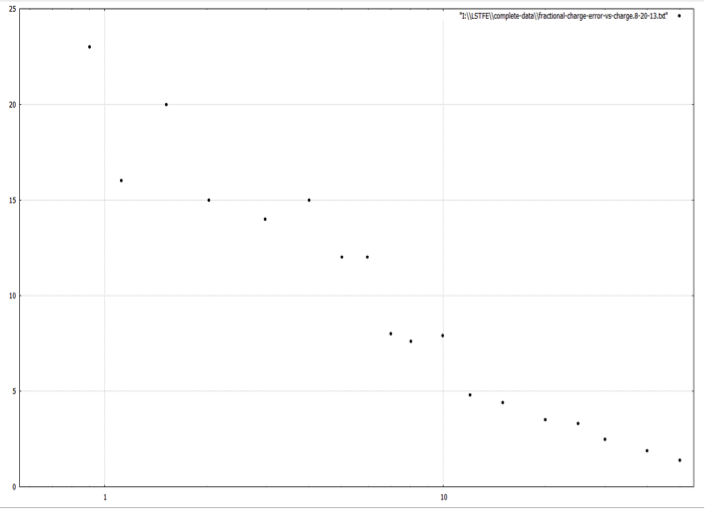
\includegraphics{Tracker/SCIPPTracking/SCIPPTracking}
\caption{Fractional pulse-height uncertainty (percent) versus injected charge (fC) for the LSTFE front-end ASIC.
The development of this ASIC has been done solely at the Santa Cruz Institute for Particle Physics (SCIPP) within the University of California at Santa Cruz, and while slowed significantly due to the loss of support for Linear Collider Detector R\&D, continues within SCIPP. Tasks that remain in developing a chip suitable for use in a Linear Collider Detector include the development of the digital back end; significant progress has already been made in defining the architecture of this section of the chip and in implementing this architecture in prototype form on an FPGA. Power cycling (switching the chip into a low-power quiescent mode for most of the 199 ms between beam crossings) also needs to be implemented.}
\end{figure}
 

References
[1] J. K. Carman et al., Longitudinal Resistive Charge Division in Multi-Channel Silicon Strip Sensors, Nulcear Inst. and Methods in Physics Research A579 (2007), pp 595-598.
[2] K. Collier et al., Microstrip Electrode Readout Noise for Load-Dominated Long Shaping-Time Systems, Nuclear Inst. and Methods in Physics Research, A729 (2013), pp. 127-132.

\section{KPIX}
\subsection{Introduction}
KPiX is a 1024 channel ``System on a Chip'' intended for bump bonding to large area Si sensors, enabling low multiple scattering Si strip tracking and high density Particle Flow calorimetry for SiD at the International Linear Collider (ILC).

Each channel consists of a dynamically switchable gain charge amplifier; shaping; threshold discrimination; and 4 sample and hold capacitors and 4 timing registers. The chip permits 4 separate measurements of amplitude and time of threshold crossing during each train, and amplitude digitization and readout during the intertrain period. The dynamic range is from sub minimum ionizing particle (mip) (in \unit[320]{\micron} silicon) to more than 2000 mip. KPiX also has a calibration system for each channel, servos for leakage compensation, ``DC'' reset for asynchronous operation for testing with cosmic rays, and polarity inversion for use with GEMs and similar detectors. The noise floor is about \unit[0.15]{fC} ($\simeq$ 1000 electrons), and the maximum signal is \unit[10]{pC} (utilizing the dynamic range switching). The full dynamic range corresponds to 17 bits.

\subsection{Recent Milestones}
ILC related R\&D in the US is largely unfunded and small efforts are being kept alive on the margins. The KPiX R\&D is such an example of necessary work for SiD that is marginally alive.
\subsection{Engineering Challenges}
At this time, KPiX is seen as the baseline readout system for the tracker and electromagnetic calorimeter. A stack of 13 EMCal sensors with bump bonded KPiX was assembled for a beam test at SLAC in the summer of 2013. That test discovered that two kinds of crosstalk are significant:
\begin{itemize}
	\item In-time crosstalk occurs due to parasitic coupling of traces on metal 2 of the sensor to other pixels. The level of crosstalk increases with the size of the signal, and decreases with increased speed of the front end charge amplifier (meaning increased current and power dissipation).  A new sensor design is being developed that uses metal 1 to shield the traces of metal 2, and these ideas will be tested in the next sensor prototype.
	\item Out-of-time cross talk occurs when many pixels are hit and reset simultaneously. The resets collectively cause other pixels to trigger, and a cascade builds up. This uses up all the KPiX buffers. The root cause of the problem appears to be some internal logic within KPiX that is not current limited, and will require design modification.
\end{itemize}
A more general issue is that both the EMCal and tracker sensors from Hamamatsu were ordered with Al pads, as it was believed that plating (by the zincate process) a stack of metals culminating with Au would be straightforward. This turns out to be wrong. %After many attempts at University of California Davis (UCD) and local industry, IZM  has Ar ion etched the pad surfaces and sputtered a base layer, permitting the buildup of a stack that ended with Au, and permitting the attachment with solder bumps that had been placed during KPiX manufacture by TSMC. Testing of these sensors revealed $\approx 10$\% pixel to pixel shorts and some opens of signal traces, that are suspected to be damage caused by the Ar ion etch. 
Future sensors will be ordered with Au pads. 

An additional issue is that the Tracker sensor was planned to be wire bonded to its (very thin) cable. The sensor oxide layer is not strong enough to allow wire bonding without damage, and so must be solder bumped. The pad pitch is small, and solder bumping the cable will be challenging. The trouble with the wire bonding to the sensor was unexpected.
Another concern is that the current design of KPiX has deadtime after a pixel has accepted a trigger. Only the triggered pixel is affected; all the other pixels are available for signals. This deadtime is different from the usual notion of data acquisition deadtime where the entire detector is unavailable, but the correction to the luminosity integral is easy. Finally, the buffer requirement (4 in the current version of KPiX) is being re-evaluated in SiD simulations. A possible new architecture for KPiX is in early stages of evaluation.
A small mechanical engineering effort has started to study the structure of the EMCal. The Sid EMCal has emphasized thin gaps between the tungsten layers to minimize the Moliere radius, and this implies that the structure is connected by columns at the vertices of the sensors. The DBD design shows hexagonal sensors, which indeed are the most efficient way of tiling large areas, but no consideration was given to the edges of these arrays. The design is being re-evalutated to optimize the cost-effectiveness over the whole area taking into account geometric efficiencies and total wafer cost.
Tracker sensors are now at IZM for the pad plating and subsequent bonding of KPiX; they will then go to UCD for cable attachment and testing.
\subsection{Future Plans}
Assuming positive developments with Japan are announced soon, we expect the financial support to improve. It should be noted that an important effect of the withdrawal of support is that most of the US collaborators have been forced to move to other work. 
\begin{itemize}
	\item EMCal Sensors: A second round of prototypes will be designed and ordered with rectangular layout; shielded traces, and Au pads.
	\item Tracker Sensors: The current prototypes will be evaluated, and if appropriate tested in a beam.
	\item KPiX: A new architecture with little (or no) deadtime will be evaluated. A decision will be made to develop this new architecture or incrementally.
	\item improve the existing design.
	\item The EMCal mechanical structure will be pushed towards a conceptual design.
\end{itemize}
\subsection{Applications Outside of Linear Colliders}
This work represents a significant step in the aggressive integration of silicon sensors with readout electronics, just short of integrating the electronics directly into the sensors. It has prompted consideration of this approach by CMS for calorimetry and by ATLAS for a muon system.  It may have applications in sensors for light sources as well as other particle physics detectors.

\section{Time Projection Chamber -- Bonn}
\subsection{Collaborating Institutions}
\begin{itemize}
	\item CEA Saclay
	\item NIKHEF
	\item Fraunhofer Institut IZM, Berlin
\end{itemize}
\subsection{Introduction}
The University of Bonn is studying the pixelized readout of a TPC for the ILD detector. The readout is based on the Timepix ASIC with a triple GEM or Micromegas based gas amplification.

\subsection{Recent Milestones}
The first studies were based on the triple GEM setup with a single Timepix chip. This readout was mounted in a small test detector in the Bonn laboratory. Here, the working principle was tested with a long drift distance. It could be demonstrated that the transverse spatial resolution of the reconstructed primary electrons was close to the expected diffusion limit of single electrons. The results are summarized in the following publications:
\begin{itemize}
\item C. Brezina et al., Operation of a GEM-TPC with pixel readout, IEEE TNS, Vol. 59, No. 6, December 2012, pp. 3221-3228
\item J. Kaminski et al., Time projection chamber with triple GEM and pixel readout, NSS Conference Record, 2008, 2926-2929
\item C. Brezina et al., A Time Projection Chamber with triple GEM and pixel readout, 2009 JINST 4 P11015
\item J. Kaminski et al., Time projection chamber with triple GEM and highly granulated pixel readout, LP 2009, Conf. Proc. C0908171 (2009) 533-535
\item P. Schade et al., A large TPC prototype for a linear collider detector, NIMA 628 (2011) 128-132
\end{itemize}

The new focus are GridPix based detectors, where the gas amplification stage is a Micromegas produced in a postprocessing technique, which guarantees a high quality grid well aligned with the readout pixels. This approach was pioneered by NIKHEF and the University of Bonn has modified the production process together with the Fraunhofer Institut IZM so that a wafer-based production of GridPix detectors is standard by now. The new GridPixes were tested on small prototype detectors and also assembled in an 8 GridPix module for the Large Prototype detector at DESY. A successful test beam campaign was performed last year.
\begin{itemize}
\item M. Lupberger, The Pixel-TPC: first results from an 8-InGrid module, 2014 JINST 9 C01033
\item W. Koppert, GridPix detectors: Production and beam test results, NIMA 732 (2013) 245–249 
\end{itemize}
The current work is focused on a new LP module with about 100 GridPixes. This module is a demonstrator that larger areas (~\unit[400]{$cm^2$}) can be produced and operated. It shall be tested in the LP at the beginning of next year. For this a number of challenges have to be coped with. In particular commercial readout systems are not easily scalable. This is why Bonn has developed a cheap and easily expandable system based on the Scalable Readout System (SRS) of the RD51 collaboration.
In addition Bonn is developing the software for reconstructing and analyzing the test beam and simulation data. For this the LCTPC software framework of MarlinTPC is used.
\begin{itemize}
\item J. Abernathy et al., MarlinTPC: A Common Software Framework for TPC Development, NSS conference record, 2008, 1704-1708
\end{itemize}
Finally, Bonn also takes part in designing new pixel chips. To test the new digitization and readout techniques two test chips were designed in collaboration with N'IKHEF. Then Bonn also contributed to the design of the Timepix successor chip, Timepix3, which is being tested now:
\begin{itemize}
\item A. Kruth et al., GOSSIPO-3: measurements on the prototype of a read-out pixel chip for Micro- Pattern Gaseous Detectors, 2010 JINST 5 C12005
\item C. Brezina et al., GOSSIPO-4: Evaluation of a Novel PLL-Based TDC-Technique for the Readout of GridPix-Detectors, IEEE Trans. Nucl. Sci. Vol. PP
\item Y. Fu et al., The charge pump PLL clock generator designed for the 1.56 ns bin size time-to-digital converter pixel array of the Timepix3 readout ASIC, 2014 JINST 9 C01052
\end{itemize}

\subsection{Engineering Challenges}
The production of a module with 100 GridPixes requires 4 main components: The production of a
large number of GridPixes with sufficiently good quality. This has been addressed by the new production method and a large batch is being produced. The challenge of the readout is being addressed by the new readout system. Finally the distribution of the LV power to all ASICs and the cooling of the ASICs still are unclear, but since both challenges are similar for most readout electronics, standard solutions are expected to be adequate.

\subsection{Future Plans}
On a short term the production of the 100 ASIC module is the main goal at Bonn. If this module has been successfully operated, we are interested in replacing the Timepix ASIC by the Timepix3 ASIC and produce GridPix detectors with this improved chip. There are also some ideas of how to improve the grid structure and make it more reliable. Finally, the reconstruction and analysis software needs further improvement and has to be extended, so that simulated data for the final TPC (i.e. 10,000 hits per track) can be studied.

\subsection{Applications Outside of Linear Colliders}
A single InGrid detector will be installed this year in the CAST experiment for axion search. For a CLIC-TPC a highly granular (i.e. pixelized) readout structure is mandatory to lower the occupancy.

\section{Electromagnetic Calorimeter R\&D}
\section{Scintillator Strips}
\subsection{Introduction}

The CALICE scintillator strip-based ECAL (ScECAL) uses a scintillator  strip
structure to deliver the granularity and resolution required of an ILC detector.
Each strip is individually read out by a Multi Pixel Photon Counter (MPPC, a
silicon photon detector produced by Hamamatsu Photonics K\.K\.~\cite{Gomi:2007zz}). Although
plastic scintillators have been widely used in calorimeters, this is the first
time that a highly granular calorimeter has been made using scintillator strips.
Such an ECAL has a smaller cost than alternative technologies using silicon
sensors (e.g.~\cite{1748-0221-3-08-P08001}). The MPPC has promising properties for the ScECAL: a small
size (active area of $\unit[1 \times 1]{mm^2}$ in a package of $\unit[2.4 \times 1.9 \times 0.85]{mm^3}$), excellent
photon counting ability, low cost and low operation voltage ($\unit[70]{V}$), with
disadvantages of temperature-dependent gain, saturation at high light levels,
and the dark noise rate. The use of tungsten absorber material
minimises the Moliere radius of the calorimeter, an important aspect for the
effective separation of particle showers required by PFA reconstruction. The
chosen strip geometry allows a reduction in the number of readout channels,
while maintaining an effective granularity given by the strip width, by the use
of appropriate reconstruction algorithms. One such algorithm, know as the Strip
Splitting Algorithm~\cite{Kotera2015}, has been developed and demonstrated to perform well in
jets expected at ILC.

\subsection{Recent Milestones}
\begin{itemize}
	\item introducing a new scintillation light readout scheme, with different scintillator strip shape by having better homogeneity
	\item photo-sensor of increased number of pixels in $\unit[1]{mm}\times\unit[1]{mm}$, this leads larger dynamic range for the calorimeter
	\item more experience on the FE read out board and ASICs
\end{itemize}
They are not published yet, instead some proceedings

\subsection{Engineering Challenges}
\begin{itemize}
	\item wrapping the scintillator strip and align them on the FE read out layer automatically
	\item mass test facility for the read out layer
\end{itemize}

\subsection{Future Plans}
\begin{itemize}
	\item deciding on the scintillator layer: shape of scintillator strip, how to read out scintillation light, the location of  photo-sensor, size and shape of photo-sensor and mass production scheme
	\item developing photo-sensor with Hamamatsu photonics company, to have lager dynamic range and mass test scheme
	\item establish a detector fabrication plan
\end{itemize}

\subsection{Applications Outside of Linear Colliders}
\begin{itemize}
	\item photo-sensor named MPPC from Hamamatsu Photonics KK is employed for the T2K experiment, CMS upgrade (HC-CAL), Belle II detector (end-cap muon)
	\item PET and SPECT development
\end{itemize}

\section{Silicon-Tungsten ECAL in ILD}

\subsection{Introduction}
The silicon-tungsten electromagnetic calorimeter for ILD aims to develop a highly granular detector optimized for particle flow performance. The calorimeter uses a sandwich architecture with $5 \times \unit[5]{mm^2}$ silicon pads as active elements embedded in an alveola structure made of tungsten. The group is active in the development of simulation software and algorithms for calorimeter reconstruction, as well as engineering for the design, and fabrication of the readout chips.

\subsection{Recent Milestones}
The work is now focusing on the construction of a technological prototype. This is a new milestone after the successful operation of the ``Physics Prototype'' in the years 2004--2011, including large scale beam tests at DESY, CERN at FNAL and data analysis~\cite{Adloff:CAN025}. An analysis of data recorded in 2007~\cite{Adloff201197} gives confidence that embedding the front end electronics into the calorimeter layers does not compromise the detector performance.

For the technological prototype, the SKIROC ASIC will be embedded into the calorimeter layers and mounted on 9 layer PCBs that will be as thin as \unit[1.5]{mm}. Silicon wafers, the PCB and the 16 mounted circuits constitute the Active Signal Units or ASUs. Up to ten of these ASUs will be assembled to form a calorimeter layer. The technology of the interconnections was applied with success to first units of the technological prototype.

A series of beam tests with simplified ASUs have been carried out in the years 2012 and 2013 at DESY. The analysis of these data validated the concept of the front end electronics but will also allow for correcting a small number of shortcomings of the SKIROCs ASIC. These will be corrected in the version SKIROC2b that is supposed to be produced at the end of 2014. A paper on the analysis of the 2012 data has been submitted to JINST in March 2014.
Particularly in summer 2013 (i.e. Post-DBD phase), the SKIROC ASIC has been operated in power pulsed mode. For this bias currents of the ASIC are shut down and raised with a given frequency (\unit[5]{Hz} for ILC, \unit[10]{Hz} in our beam tests). The good agreement between the MIP spectra obtained in power pulsed and conventional mode (see e.g.~\cite{Poschl:Giessen:ECAL:2014}) give confidence that this technology can indeed be applied for a calorimeter at a linear collider and more precisely at the ILC. More studies are needed as the technological prototype grows in size.
After the departure of the OMEGA group from LAL the development of microelectronics at LAL has been stopped. A new institute with the same name, i.e. OMEGA, has been created by the IN2P3 and is hosted at the Ecole Polytechnique. The ILC group at LAL will continue to collaborate with the new institute. The details will however have to be sorted out under the new circumstances. It is maybe still worthwhile to say that for the next it is planned to first produce the debugged version SKIROC2b (see above) and then the version SKIROC3. The latter will comprise all the features needed for an ASIC.

Other recent accomplishments include:
\begin{itemize}
	\item R\&D on scalable technology for all the involved large detector aspects (integration of embedded readout chips, on thin supporting electronics boards, in self-supporting tungsten--carbon mechanical elements ensuring the cooling and protection; all made of exchangeable elements with a quality control procedure; the associated DAQ).\todo{is this completed?}
	\item \todo{date?} Realization of a large self-supporting W--Carbon fiber structure with integrated stress monitoring (using Fiber Bragg Grating)
	\item Beam tests of base sensor units of the technological prototype
	\item Submission of a paper on the analysis of 2012 beam test data to JINST~\cite{Rouene2013470},\cite{Frisson:2013:CIN023}.
	\item \todo{Recent?} Reconstruction tools adapted to the high granularity calorimeters (photon reconstruction [\todo{Reference} GARLIC], Advanced clustering [\todo{Reference} ARBOR], event displays [\todo{Reference} DRUID])
	\item Operation of SKIROC~\cite{1748-0221-6-12-C12040} in pulsed power mode (with \unit[5]{Hz} as foreseen by ILC baseline and with \unit[10]{Hz} as envisioned in high luminosity operation).
	\item SiECAL test beam experiments were carried out in Jul. 2012, Feb. and Jul. 2013 to test the SiECAL technological prototype. The front-end electronics of the prototype was integrated into an active layer to realize a highly granular calorimeter. In the 2012 test beam, we operated six layers under a continuous current mode. The achieved signal to noise ratio was greater than 10 with SKIROC2 ASICs. In the 2013 test beams, we successfully operated and took data with the prototype under a power pulsing mode. At the same time, we found several issues related to the power pulsing operation. Digital lines on the front-end electronics disrupts analog signals. We had to wait $\unit[600]{\mu s}$ for the electronics to stably take the data. We measured pedestal signals in a magnetic field, and confirmed that active channels were working in stable up to \unit[2]{T}.
\end{itemize}
As for the R\&D of silicon sensors, we measured several new samples with different guard ring types. It is known that a Si sensor makes small fake signals along with its sensor edge when a large amount of current is generated by an electromagnetic shower in a calorimeter. If the fake signal is reasonably small, we can use the Si sensor for the ILD. To test the fake signal, we introduced an infrared laser system in Kyushu University to measure the Si sensor response with a similar condition of beam test in a laboratory scale. We are setting up a multi-pixel readout system without SKIROC2 ASIC. We can then measure the intrinsic Si sensor properties with the IR laser system.
Studies on the SiECAL optimization have been performed with full ILD detector simulation. We performed simulation studies with different setting of PCB thickness, dead volume related the sensor edge, and fraction of dead channels. We found:
\begin{itemize}
	\item The PCB thickness does not change the performance of the jet energy resolution.
	\item The dead volume proportionally degrades the performance, but the current Si sensor design is acceptable.
	\item The fraction of dead channels does not much degrade the jet energy resolution up to the fraction of ~5\%.
\end{itemize}

\subsection{Engineering Challenges}
\begin{itemize}
	\item Silicon wafer cost reduction when used for calorimetry; direct contact with producers established (Hamamatsu, On-Semi, \ldots).
	\item A chip with the good dynamic, noise, power dissipation (using power pulsing), etc.
	\item Integration in a compact device, ensuring all the requests (precision: electronic and mechanic, heat production, reliability)
	\item Industrialization of solutions; scalability of tests for a 100M channel detector.
\end{itemize}

\subsection{Future Plans}
Detector R\&D plan in coming years are shown below.
\begin{itemize}
\item Test beam experiments with long SiECAL slabs using new front-end electronics with SKIROC2 ASICs,
\item Combined test beam experiments with ScECAL and AHCAL,
\item Development a DAQ system (set up of hardwares, development of software
and firmware) for the combined tests.
\item Further R\&D of silicon sensors, using the IR laser system, to determine the final design.
\item Irradiation test with several types of Si sensors.
\item Looking for Japanese companies which can produce SiECAL front-end
electronics in prospect of mass production.
\item Further optimization of SiECAL and Hybrid ECAL with full ILD detector simulation.
\end{itemize}

\subsection{Plans of the near future - Ecal assembly bench and R\&D on digital electronics}
The different units of the SiW Ecal for the ILD detector need to be assembled into detector layers of up to two meter in length comprising up to 10 detection units dubbed ASUs. For this we propose to develop an assembly line, incorporating the reception and the test of the material, the alignment of the ASUs and the interconnection, with a continuous monitoring for quality control purposes. The deliverable is a still manual assembly bench capable for a small production of layers. Based on the manual assembly bench we will propose an automatized system for mass assembly together with industrial partners. A survey to search for partners is part of the proposal. A goal is to design the system such that it can be easily duplicated at other sides. In the ideal case the assembly bench is versatile enough to reply to needs for other detector systems than ILD (e.g. CMS). Relevant data recorded during the assembly process can for example be stored in a database. The tools for efficient storage and retrieving data and information about detector components can be developed in collaboration with other proposals aiming at the mass production of calorimeter elements and/or benefit from similar tools developed e.g. for the XFEL project. This project might become a task within the calorimeter package of the AIDA2 project.


\subsection{Further Activities}
Although not explicitly asked it is worthwhile to point out that the LAL plays also a role in the integration of the ILD detector. Notably the engineers are in charge of validating the CAD Models of the sub-detectors before they come part of the official ILD database. It can be expected that this activity increases in importance when the ILC will move towards a real project.

Finally, since 2012 there is a collaboration with the AppStat group of LAL. The aim of this collaboration is to develop algorithms based on machine learning techniques to assure an optimal separation of particle showers in highly granular calorimeters.

The departure of the OMEGA group requires re-orientation of the LAL contribution to detector electronics. The LAL has recognised competences in digital electronics. It is considered to embark on the R\&D for DAQ systems for linear collider detectors. Details will be worked during 2014. It is envisaged to make this work part of the calorimeter package of the AIDA2 project.

In addition, we are working on a study of Hybrid ECAL which has ”Si sensor ”and ”Scintillator and photo sensor ”Active layers as an optimization of ECAL in few of the performance and the cost.

\subsection{Applications Outside of Linear Colliders}
\begin{itemize}
	\item CEPC, TLEP and directly today on CMS upgrade
	\item The compact Silicon-W design has been used in the PAMELA satellite (very similar to physics prototype)~\cite{1742-6596-160-1-012039}
\end{itemize}


\section{Hadronic Calorimeter R\&D}
\section{Scintillator Tiles}
\subsection{Collaborating Institutions}
\subsection{Introduction}
\subsection{Recent Milestones}
\subsection{Engineering Challenges}
\subsection{Future Plans}
\subsection{Applications Outside of Linear Colliders}

\section{Resistive Plate Chambers}

\subsection{Description of the DHCAL}
The Digital Hadron Calorimeter or DHCAL uses Resistive Plate Chambers (RPCs) as active elements. The chambers are read out with $\unit[1 \times 1]{cm^2}$ pads and 1-bit (digital) resolution. A small-scale prototype was assembled and tested in the Fermilab test beam in 2007 to validate the concept.
Based on the success of the small-scale test [1-6], a large prototype with up to 54 layers and close to 500,000 readout channels was built in 2008 -- 2011. Each layer measured approximately $\unit[96 \times 96]{cm^2}$ and was equipped with three chambers, stacked vertically on top of each other.
For tests with particle beams the DHCAL layers were inserted into a main stack of 38 or 39 layers, followed by a tail catcher with up to 15 layers. For the tests performed at Fermilab the main stack contained steel absorber plates. At CERN the absorber plates contained a Tungsten based alloy. In both cases the tail catcher featured steel absorber plates.
In the various test beam campaigns combined, spanning the years 2010 -- 2012, the DHCAL recorded of the order of 14 Million muon events and 36 Million secondary beam events, where the latter contained a mixture of electrons, muons, pions, and protons.
\subsection{Current R\&D activities}
The analysis and publication of the test beam results are currently the highest priority of the DHCAL group. Major challenges, such as the calibration (or equalization) of the response of the RPCs and the detailed simulation of the response of RPCs, are very close to having been overcome [7-11].
In parallel, to the analysis of test beam data, the group is pursuing the following R\&D activities:
\subsubsection{Development of 1--glass RPCs}
The DHCAL prototype featured a standard chamber design based on RPCs with two resistive plates. The Argonne group, however, proposes to eliminate one of the glass plates in future applications. The advantages are: close to unit pad multiplicity with significant simplification of the calibration and monitoring procedure, reduced thickness of the active element, higher rate capability, and insensitivity of the response to the surface resistivity of the resistive layer (used to apply the High Voltage). To date several 1-glass RPCs have been assembled. The chambers tested very well with cosmic rays. Tests in particle beams are planned for future test beam campaigns.
\subsubsection{Development of high-rate RPCs}
Due to the high bulk resistivity of glass (and Bakelite), RPCs are notoriously rate limited [12]. The DHCAL group is addressing this shortcoming with the development of semi-conductive glass (in cooperation with COE college) and of low-resistivity Bakelite (in co-operation with USTC). First chambers with samples of low-resistivity glass plates have been assembled and have tested in the Fermilab test beam.
\subsubsection{Development of a High-Voltage distribution system}
With up to 50 layers in a single calorimeter module, a cost-effective way to distribute the High-voltage to individual layers is required. A system capable to regulate the voltage within a few 100 V, to monitor both the current and the voltage, and to switch off individual channels, is being developed. A first prototype controlling a single channel has been assembled and tested successfully with an RPC. The development is currently on hold due to lack of funding.
\subsubsection{Development of a gas recycling system}
The operation of RPCs requires a gas mixture, which is both costly and environmentally harmful. To limit the effect of releasing gas into the environment, the DHCAL group is developing a gas recycling system. The system is based on a new approach, appropriately labeled ``Zero Pressure Containment''. A prototype of the gas collection subsystem is currently being assembled; however, progress is again slow due to lack of funding.
\subsubsection{Development of the next generation front-end readout system}
The next generation front-end readout system will contain several upgrades compared to the current system: higher channel count, token ring passing, low power operation, power pulsing, and improved internal charge injection systems. To proceed, the project is awaiting funding from both US and Chinese agencies.

\subsection{Engineering challenges}
Several engineering challenges remain to be addressed before an RPC-based DHCAL can be proposed as an option for a colliding beam detector. Following is an (incomplete) list of the major issues:
\begin{itemize}
\item Industrialization of the construction of RPCs.
\item Design of the readout boards, covering the entire area of the layer (with varying width). The design is expected to feature only a minimum number of different boards.
\item Design of the gas distribution system, which ensures equal pressure in all layers of a given module, independent of its orientation.
\item Development of a cooling strategy for the front-end boards, which will include power pulsing, as well as active cooling.
\item Development of a module assembly procedure.
\end{itemize}

\subsection{Plans for the coming years}
The activities of the coming years depend strongly on the progress with the Japanese intentions to host the ILC. Assuming the ILC project goes ahead, the DHCAL group will
a)  Complete the analysis and publication of the test beam data,
b)  Complete the R\&D projects listed above, and
c)  Start the development of the design of calorimeter modules.
In case, the ILC is not going forward, the group plans on completing the data analysis and to continue the tests of high-rate RPCs. Other R\&D projects, such as the development of distribution systems, will be put on hold.

\subsection{Applications beyond the ILC}
The DHCAL technology was specifically developed for the hadron calorimeter of the ILC, with its low particle rate and radiation dose. To export the technology to other environments, the rate capability of the chambers and the radiation hardness of the readout need to be improved. The former is being addressed with low-resistivity plates (glass and Bakelite), while the latter will require a new front-end readout system based on an ASIC using a smaller feature size. Possible applications are the tail catcher of the forward calorimeters of CMS and the outer wheels of the ATLAS muon system. Both options are being pursued actively.

References
\begin{enumerate}
\item \fullcite{Drake200788}
\item \fullcite{1748-0221-3-05-P05001}
\item \fullcite{1748-0221-4-04-P04006}
\item \fullcite{1748-0221-4-06-P06003}
\item \fullcite{1748-0221-4-10-P10008}
\item \fullcite{1748-0221-5-02-P02007}
\item \fullcite{Repond:2011:CAN30}
\item \fullcite{Repond:2013:CAN30A}
\item \fullcite{Xia:2011:CAN31}
\item \fullcite{Xia:2011:CAN32}
\item \fullcite{Repond:2012:CAN39}
\item \fullcite{Bilki:2013:CAN42}
\item \fullcite{Xia:2014:RPC2014}
\end{enumerate}

\section{GEM}
\subsection{Introduction}
The group pursues the development of Gas Electron Multiplier technology for instrumenting a digital hadronic calorimeter (DHCAL) at the ILC. The 
\subsection{Recent Milestones}
\subsection{Engineering Challenges}
\subsection{Future Plans}
\begin{itemize}
\item To be determined
\end{itemize}
\subsection{Applications Outside of Linear Colliders}

\section{FCAL}
\subsection{Introduction}
Two special calorimeters are foreseen in the very forward regions of a linear collider detector, denoted hereafter as
LumiCal and BeamCal.
These calorimeters will deliver both a fast and a precise measurement of the luminosity
and extend the detector coverage to low polar angles,
important e.g. for new particle searches with missing energy signature.
Detailed Monte Carlo studies have been performed in all member institutes to
optimize the design of the calorimeters, estimate the background from physics processes and understand the impact
of beam-beam interactions on the luminosity measurement~\cite{2010JInst...512002A}.
A sketch of the design is shown in Figure~\ref{fig:Forward_structure}~(left).
To ensure a high efficiency for single high energy electron detection on top of the large and widely spread
background from beamstrahlung \todo{why compact? What does this mean? Moliere radius? outer radius?} very compact calorimeters are needed. In addition, compact calorimeters facilitate
the reconstruction of Bhabha scattering events.
\begin{figure}[hbp]
  \centering
   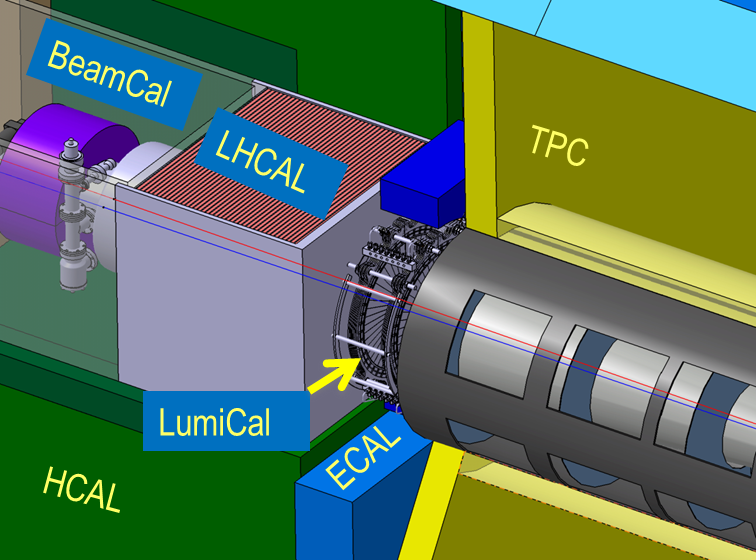
\includegraphics[width=0.45\columnwidth]{Calorimeter/FCAL/figs/forward_region_new} \hfill
   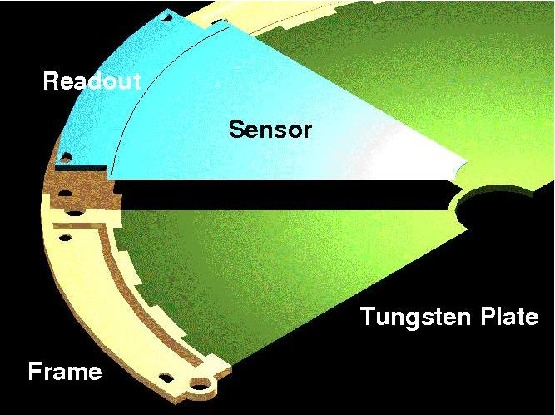
\includegraphics[width=0.45\columnwidth]{Calorimeter/FCAL/figs/BClayer}
  \caption{Left: The very forward region of the ILD detector.
  LumiCal, BeamCal and LHCAL are carried by
  the support tube for the final focusing quadrupole QD0 and the beam-pipe.
  TPC denotes the central track chamber, ECAL the electromagnetic and
  HCAL the hadron calorimeter.
  Right: A half layer of an absorber disk with a sensor sector and front-end electronics.}
  \label{fig:Forward_structure}
\end{figure}
Due to the high occupancy originating from beamstrahlung and two-photon processes,
both calorimeters need a dedicated fast readout.
In addition, the lower polar angle range of BeamCal is exposed to a large flux
of low energy electrons, resulting in depositions up to one
MGy per year. Hence, radiation hard sensors are needed.

\subsection{Mechanical Concept}
Since in both calorimeters a robust electron and photon shower measurement
is essential, a small Moli\`{e}re radius will be preferable.
Compact
cylindrical sandwich
calorimeters using tungsten absorber disks of one radiation length thickness, interspersed with
finely segmented silicon (LumiCal) or GaAs (BeamCal) sensor planes, as sketched in
Figure~\ref{fig:Forward_structure}~(right),
are found
to match the requirements from physics~\cite{2010JInst...512002A}.

\subsection{Recent Milestones}
\subsection{Engineering Challenges}
Engineering challenges within the current and future research within FCAL are the following:
\begin{itemize}
\item{a slim assembled sensor plane. The space between absorber planes must be kept as small
as possible. The fan-out to move the signals from the sensor pads to the outside radius must be very thin and
hence a new connectivity technology must be applied.}
\item{multichannel front-end and ADC ASICs for the prototype.
A compromise must be found between integration, miniaturization and costs}.
\item{operation using \todo{what is the challenge?} power pulsing}.
\item{a dedicated solution for data concentration, \todo{be more specific} data reduction and transmission}.
\item{\todo{be more specific} precise alignment and position monitoring}.
\end{itemize}

\subsection{Future Plans}

\subsubsection{Sensors and ASICs}
Large area GaAs sensors, as shown in Figure~\ref{fig:GaAs}, were developed
and produced in collaboration with partners in industry. The Liquid Encapsulated
Czochralski technology is used. The sensors were
doped by a shallow donor (Sn or Te),
and then compensated  with Chromium.
\begin{figure}[hbp]
\begin{center}
    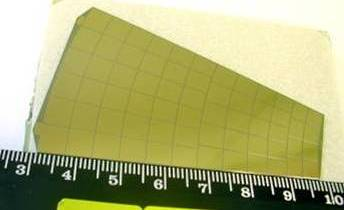
\includegraphics[width=0.8\columnwidth]{Calorimeter/FCAL/figs/GaAs_sensor_new.jpg}
  \end{center}
          \caption{A GaAs pad sensor developed for BeamCal.}
    \label{fig:GaAs}
\end{figure}
This results in a semi-insulating GaAs material with a resistivity of about $\unit[10^7]{\Omega m}$.
The sensors are \unit[0.5]{mm} thick with pads of a few mm$^2$ area. The operation voltage is about \unit[100]{V} with
leakage current per pad less than \unit[500]{nA}.

Prototypes of LumiCal sensors have been designed
and manufactured by Hamamatsu
Photonics.
Their shape is a ring segment of 30$^\circ$.
The thickness of the n-type silicon bulk is \unit[0.320]{mm}.
The pitch of the concentric p$^+$ pads is \unit[1.8]{mm} and
the gap between two pads is \unit[0.1]{mm}.
The bias voltage for full depletion ranges between 39 and \unit[45]{V},
and the leakage currents per pad are below \unit[5]{nA}~\cite{eudet2009}.

Dedicated ASICs were designed choosing
an
architecture~\cite{Boie1982365,Gatti:1986qq}
comprising a charge sensitive amplifier and a shaper.
ASICs, containing 8 front--end channels, were designed and fabricated in $\unit[0.35]{\micron}$ CMOS technology.
A micro-graph of the prototype, glued and bonded on the PCB, is shown Figure~\ref{fig:frontend_photo}.
A variable gain in both the charge amplifier and
the shaper is implemented by a mode switch. The peaking time of the shaper output signal is \unit[60]{ns}.
More results of the measurements of the performance were published elsewhere~\cite{4600902}.
A dedicated low-power, small-area, multichannel ADC is designed and produced~\cite{6156491}.
\begin{figure}[hbp]
\begin{center}
 \begin{tabular}{rrr}
    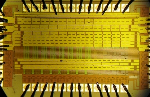
\includegraphics[width=0.4\columnwidth]{Calorimeter/FCAL/figs/fcal_lumical_fe_photo}
     &~~~~~~&
 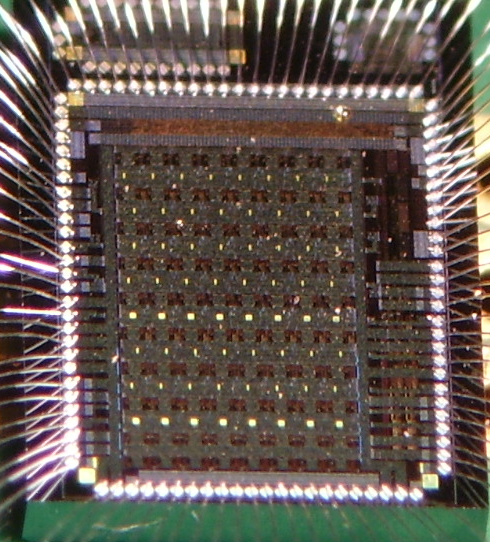
\includegraphics[width=0.4\textwidth,height=0.28\textwidth]{Calorimeter/FCAL/figs/adc_asic_photo.png} \\

\end{tabular}
   \end{center}
          \caption{Left: Micrograph of front--end ASIC.
               Right: Micrograph of ADC ASIC.}
    \label{fig:frontend_photo}
\end{figure}
It comprises eight 10-bit power and frequency (up to \unit[24]{MS/s}) scalable pipeline ADCs and the necessary
auxiliary components.
A micro-graph of the prototype is shown in Figure~\ref{fig:frontend_photo}.

A dedicated ASIC development is ongoing for BeamCal~\cite{6200898}
with a special option for a fast readout of an reduced amount of
information from each bunch-crossing to be used for a fast feedback system for beam-tuning.
A prototype of a pixel sensor readout for the pair monitor, positioned in front of BeamCal was designed in SoI
technology~\cite{Sato201153}.

\subsection{Test-beam Results}
Several test-beam campaigns were done to investigate the performance of single fully instrumented sensor planes,
both for LumiCal and BeamCal.
Prototypes of sensor planes assembled with FE and ADC ASICs,
as shown in Figure~\ref{fig:fcal_lumical_module_photo},
were built using LumiCal and BeamCal sensors~\cite{1748-0221-7-01-T01004}.
\begin{figure}[hbp]
\centering
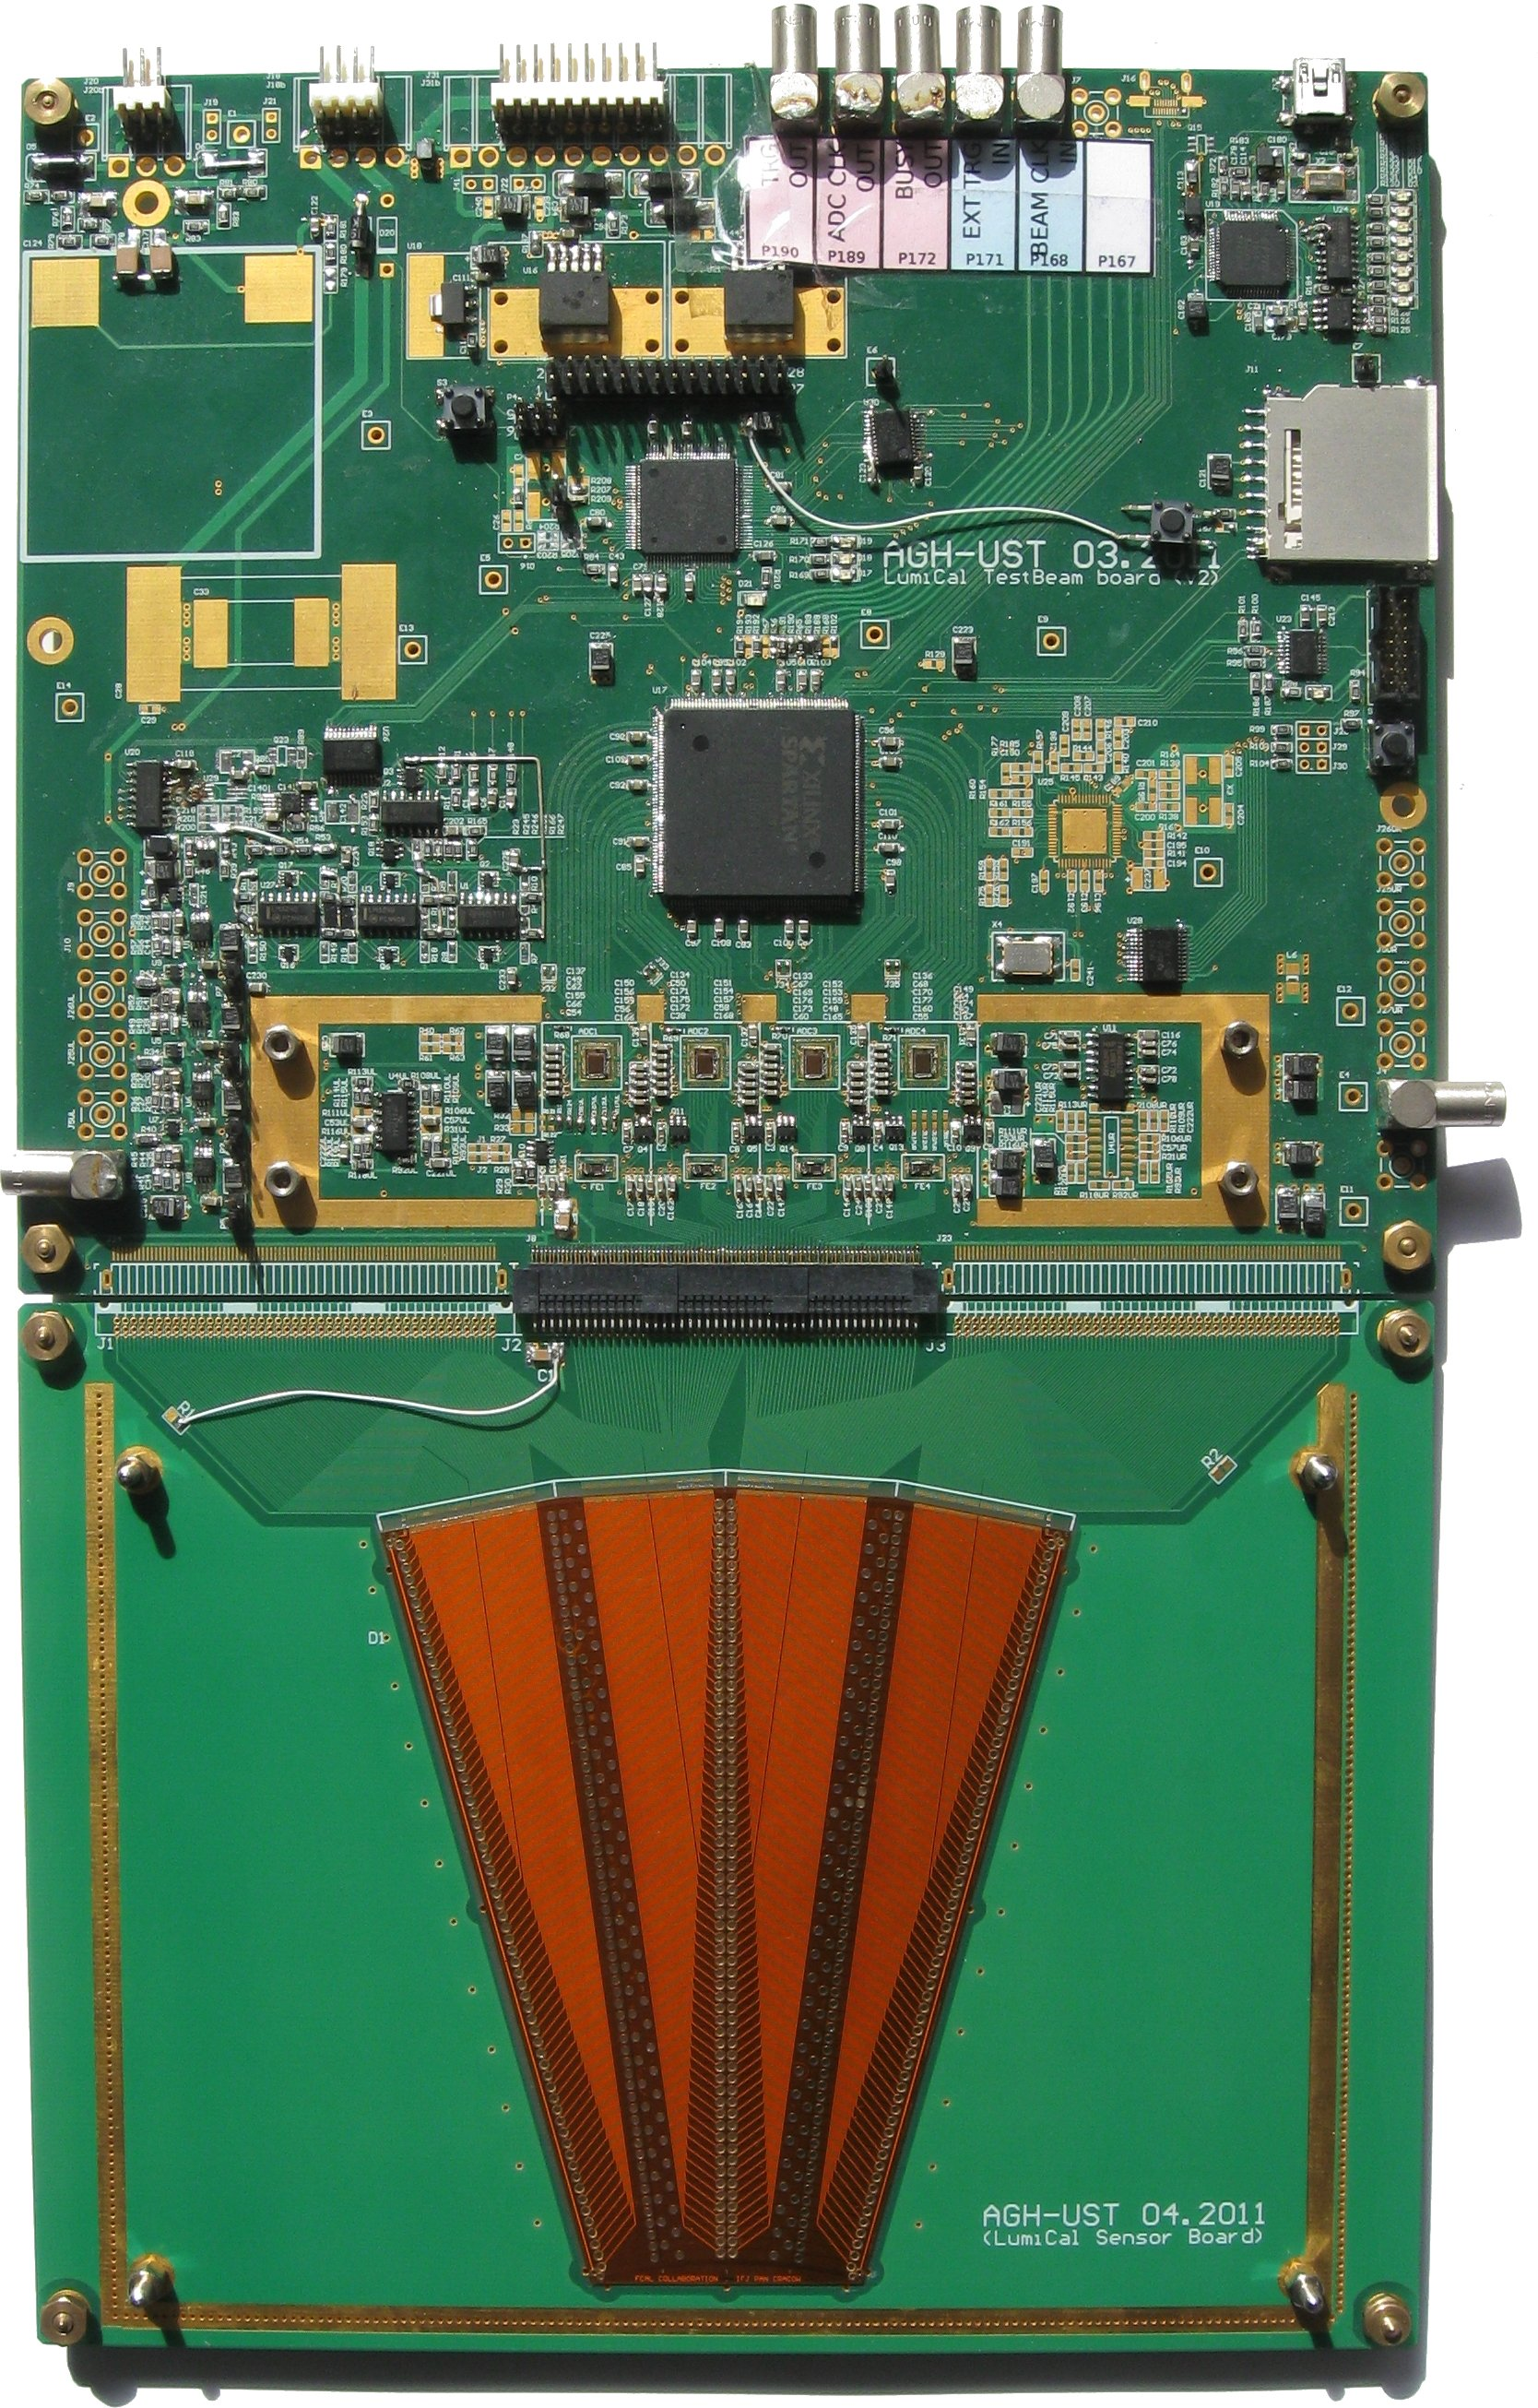
\includegraphics[width=0.35\columnwidth,angle=90]{Calorimeter/FCAL/figs/tb3_complete_module}
\caption{Photograph of LumiCal readout module with sensor connected.}
\label{fig:fcal_lumical_module_photo}
\end{figure}
The detector plane prototypes were installed in an electron beam and
the trajectories of beam particles were measured by four planes of a silicon strip
telescope.
The front-end electronics outputs were sampled synchronously with the
beam clock, a mode used at the ILC.
\begin{figure}[htpb]
\centering
  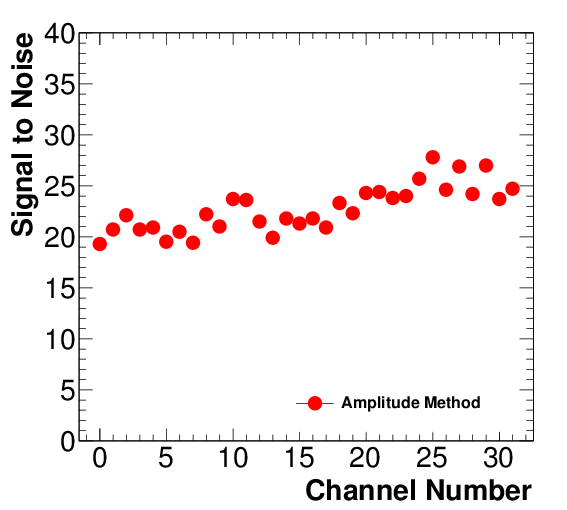
\includegraphics[width=0.45\columnwidth]{Calorimeter/FCAL/figs/StoN_AmplitudeMethod_TB11} \hfill
  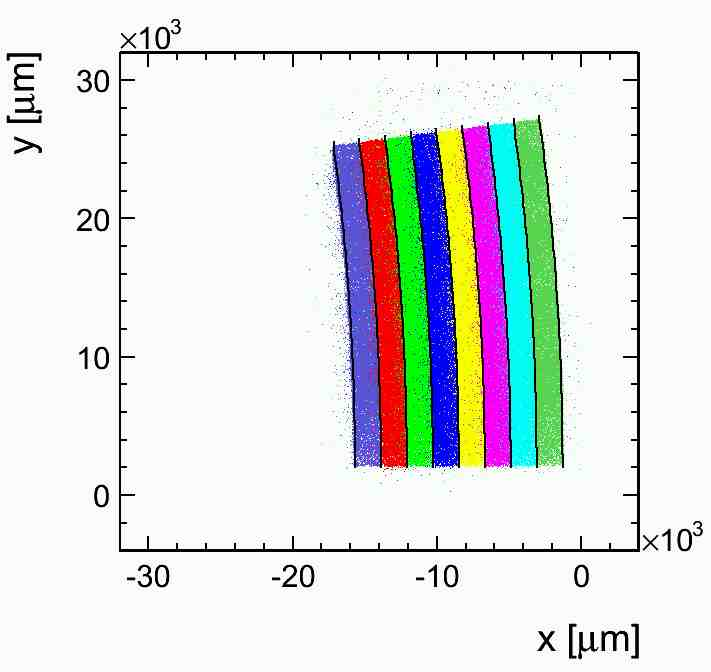
\includegraphics[width=0.45\columnwidth]{Calorimeter/FCAL/figs/hit_map_area1}
  \caption{Left: The signal-to-noise ratio of all readout channels.
          Right: Distribution of the predicted impact points on pads with a color coded signal.}
\label{fig:sinalnoise}
\end{figure}
Data were taken for different pads and also for regions covering pad boundaries.
Signal-to-noise ratios
of better than 20 are measured for beam particles both for LumiCal and BeamCal sensors,
as illustrated in Figure~\ref{fig:sinalnoise}~(left).
The impact point on the sensor is reconstructed from the telescope information.
Using a color code for the signals on the pads
the structure of the sensor becomes nicely visible, as also seen in Figure~\ref{fig:sinalnoise}~(right).
The sensor response was found to be uniform over the pad area and to drop by about 10\% in the
area between pads.

\subsection{Radiation Damage Studies}


Two studies of the radiation tolerance of potential BeamCal sensors have been carried out. The
radiation tolerance of prototype GaAs sensors has been explored by exposing the sensors
to direct irradiation from a high-intensity electron beam of about \unit[10]{MeV}~\cite{sdalinac},
which is an energy expected from beamstrahlung
remnants at the ILC.
It was found that the sensors can be operated up
to approximately \unit[1]{MGy} of this type of radiation without a significant increase in the
leakage current~\cite{1748-0221-7-11-P11022}; however, significant loss in the response to ionizing particles was observed.
In addition, several different silicon-diode sensor technologies were exposed to varying levels
of radiation induced by the SLAC End Station A Test Beam (ESTB).
For this study, the ESTB test beam, with energies
varying between 3 and \unit[11]{GeV}, was directed into a tungsten beam stop.
The beam stop was split at approximately shower-max and the sensor inserted,
leading to an exposure incorporating the full spectrum of particle species that will
irradiate the BeamCal sensors. Both n-type bulk oxygenated float-zone and magnetic Czochralski
detectors were explored, with exposures varying from 0.2 to \unit[2.2]{MGy} as allowed by
the limited exposure rate and
beam availability. It was found that, after allowing for a short period of controlled annealing,
all sensor types withstood the maximum dose that they received with little loss in response
to ionizing particles~\cite{2014arXiv1402.2692B}, but with some increase in leakage current. Further annealing studies,
geared towards achieving a minimal post-irradiation leakage current, continue.
Further irradiation studies in the ESTB are planned for the \todo{update?} spring running periods of 2014 and 2015.
The sensor assessment (``charge-collection efficiency'') apparatus at the Santa Cruz Institute
for Particle Physics is being adapted for the evaluation of pad sensors, which will allow for radiation
damage studies of the prototype GaAs sensors in this realistic electromagnetic shower environment.
Studies to push the silicon diode sensors to higher levels of irradiation are also planned.


\subsection{Technological Prototype}

Currently the goal of FCAL is to prepare a calorimeter prototype for test-beam measurements. These measurements
are essential firstly to develop and test engineering solutions to build a very compact calorimeter and
secondly to verify the results of Monte Carlo studies. Depending on the test beam
results the calorimeter may be redesigned.
For the prototype calorimeter
a mechanical structure, a sufficient amount of front-end and ADC ASICs, FPGAs for
data concentration and
a data acquisition system are needed.

\subsubsection{Mechanical Stack}

A flexible mechanical structure, as shown in  Figure~\ref{fig:mechanical_structure}, has been built as part of the AIDA I project at CERN,
to compose a calorimeter prototype instrumented both with LumiCal and BeamCal sensors. Tungsten absorber plates, glued on a permaglass
frame, are precisely
positioned on a rod assembly, and interspersed with fully assembled sensor planes.
\begin{figure}[hbp]
\centering
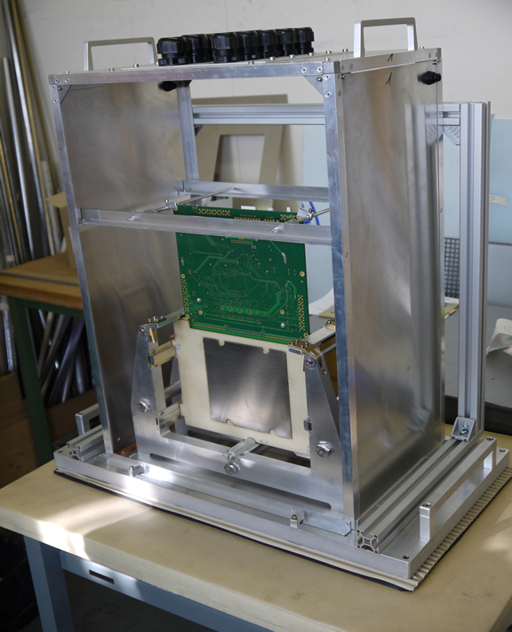
\includegraphics[width=0.6\columnwidth,]{Calorimeter/FCAL/figs/mechanical_structure_2}
\caption{Photograph of the flexible mechanical structure. Tungsten absorber plates, glued on perma-glass frames, are put into slots of the
rod assembly.}
\label{fig:mechanical_structure}
\end{figure}
The flatness of the absorber plates is better than \unit[50]{\micron} to allow high compact packing of sensor and absorber planes.

\subsubsection{Alignment and Position Monitoring }

A laboratory set-up for position monitoring has been constructed by IFJPAN Cracow using semi-transparent
silicon sensors. Test measurements demonstrated that position monitoring with \micron precision is possible.

\subsubsection{Front-End and ADC ASICs}


To match the requirements of extremely low power consumption and taking into account possible radiation
fields in the very forward region, a new development of the front-end and ADC ASICs in deep sub-micron
\unit[130]{nm} CMOS technology has been
pursued within AIDA by UST Cracow.
These ASICs will be sufficiently fast to be used both in LumiCal and BeamCal.
The overall readout architecture, so far successfully produced in \unit[350]{nm} CMOS technology and used in the test-beam
measurements as described above, has not been changed and comprises separated front-end
and ADC ASICs for each readout channel.
\begin{figure}[hbp]
\centering
    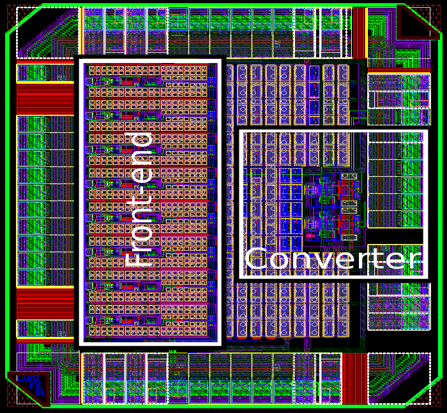
\includegraphics[width=0.45\textwidth]{Calorimeter/FCAL/figs/FE_ASIC.png} \hfill
	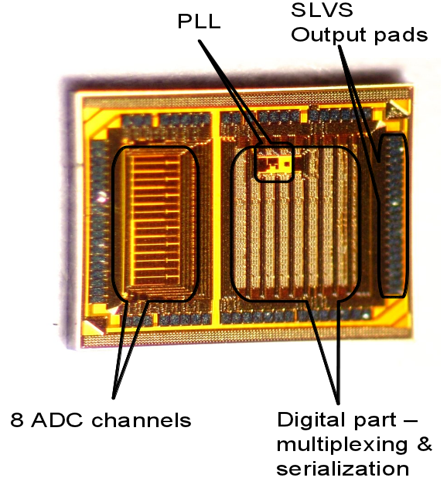
\includegraphics[width=0.45\textwidth]{Calorimeter/FCAL/figs/ADC_ASIC_2.png}
	\caption{Left: 8 channel FE ASIC in \unit[130]{nm} technology.
		 	 Right: ADC ASIC in \unit[130]{nm} technology.}
    \label{fig:ASIC_ADC}
\end{figure}
For both FE and ADC ASICs prototypes, shown in Figure~\ref{fig:ASIC_ADC}, are under test.

\subsubsection{Data Concentrator and DAQ}

In order to operate a large amount of sensor planes the readout has to be orchestrated.
For this purpose a FPGA based data concentrator is foreseen
which may deliver data in the so called AIDA protocol. The design of this device is currently under discussion.
The higher level DAQ will depend on the functionality of the data concentrator.
For the readout of test-beam data we have software, mainly developed by University of Tel Aviv,
which can be easily adopted.
For a final device FCAL will follow the developments of a common DAQ for all subdetetors.


\subsection{Applications Outside of Linear Colliders}

The expertise acquired within FCAL for radiation hard sensors and fast front-end electronics was
used to build, commission and operate fast
beam-conditions monitors at the CMS experiment at LHC.
Radiation hard sensors developed within FCAL are used as beam-loss monitors
with excellent time resolution at FLASH and LHC. A design for beam-loss monitors for XFEL is prepared.
In addition, front-end ASICs are under development for the upgrade of the LHCb tracker.

\end{document}